% One-page layout: (proof-)reading on display
%%%% \documentclass[11pt,oneside,a4paper]{book}
% Two-page layout: final printing
\documentclass[11pt,twoside,a4paper]{book}   
%=-=-=-=-=-=-=-=-=-=-=-=--=%
% The user of this template may find useful to have an alternative to these 
% officially suggested packages:
\usepackage[czech, english]{babel}
\usepackage[T1]{fontenc} % pouzije EC fonty 
% pripadne pisete-li cesky, pak lze zkusit take:
% \usepackage[OT1]{fontenc} 
\usepackage[utf8]{inputenc}
%=-=-=-=-=-=-=-=-=-=-=-=--=%
% In case of problems with PDF fonts, one may try to uncomment this line:
%\usepackage{lmodern}
%=-=-=-=-=-=-=-=-=-=-=-=--=%
%=-=-=-=-=-=-=-=-=-=-=-=--=%
% Depending on your particular TeX distribution and version of conversion tools 
% (dvips/dvipdf/ps2pdf), some (advanced | desperate) users may prefer to use 
% different settings.
% Please uncomment the following style and use your CSLaTeX (cslatex/pdfcslatex) 
% to process your work. Note however, this file is in UTF-8 and a conversion to 
% your native encoding may be required. Some settings below depend on babel 
% macros and should also be modified. See \selectlanguage \iflanguage.
%\usepackage{czech}  %%%%%\usepackage[T1]{czech} %%%%[IL2] [T1] [OT1]
%=-=-=-=-=-=-=-=-=-=-=-=--=%

%%%%%%%%%%%%%%%%%%%%%%%%%%%%%%%%%%%%%%%
% Styles required in your work follow %
%%%%%%%%%%%%%%%%%%%%%%%%%%%%%%%%%%%%%%%
\usepackage{graphicx}
%\usepackage{indentfirst} %1. odstavec jako v cestine.
\usepackage{setspace}
\usepackage[hyphens]{url}
\usepackage{pgfplots}
\usepackage{forest}
\usepackage{float}
\usepackage{nameref}

\usepackage{tabularx}

\usepackage{misc/k336_thesis_macros} % specialni makra pro formatovani DP a BP
 % muzete si vytvorit i sva vlastni v souboru k336_thesis_macros.sty
 % najdete  radu jednoduchych definic, ktere zde ani nejsou pouzity
 % napriklad: 
 % \newcommand{\bfig}{\begin{figure}\begin{center}}
 % \newcommand{\efig}{\end{center}\end{figure}}
 % umoznuje pouzit prikaz \bfig namisto \begin{figure}\begin{center} atd.

\newcommand\TypeOfWork{Master's Thesis}   \typeout{Master's Thesis} 
\newcommand\StudProgram{Open Informatics}
\newcommand\StudBranch{Software Engineering}

%%%%%%%%%%%%%%%%%%%%%%%%%%%%%%%%%%%%%%%%%%%%
% Vyplnte nazev prace, autora a vedouciho
% Set up Work Title, Author and Supervisor
%%%%%%%%%%%%%%%%%%%%%%%%%%%%%%%%%%%%%%%%%%%%

\newcommand\WorkTitle{Multi-platform Scalable Messaging System}
\newcommand\FirstandFamilyName{Bc. Oscar Hernández}
\newcommand\Supervisor{Ing. Martin Mudra}

% Pouzijete-li pdflatex, tak je prijemne, kdyz bude mit vase prace
% funkcni odkazy i v pdf formatu
\usepackage[
pdftitle={\WorkTitle},
pdfauthor={\FirstandFamilyName},
bookmarks=true,
colorlinks=true,
breaklinks=true,
urlcolor=red,
citecolor=blue,
linkcolor=blue,
unicode=true,
]
{hyperref}

\usepackage{listings}
\usepackage{color}

\definecolor{dkgreen}{rgb}{0,0.6,0}
\definecolor{gray}{rgb}{0.5,0.5,0.5}
\definecolor{mauve}{rgb}{0.58,0,0.82}

\lstset{frame=tb,
  language=Java,
  aboveskip=3mm,
  belowskip=3mm,
  showstringspaces=false,
  columns=flexible,
  basicstyle={\small\ttfamily},
  numbers=none,
  numberstyle=\tiny\color{gray},
  keywordstyle=\color{blue},
  commentstyle=\color{dkgreen},
  stringstyle=\color{mauve},
  breaklines=true,
  breakatwhitespace=true,
  tabsize=3
}

\begin{document}

%%%%%%%%%%%%%%%%%%%%%%%%%%%%%%%%%%%%%
% Zvolte jednu z moznosti 
% Choose one of the following options
%%%%%%%%%%%%%%%%%%%%%%%%%%%%%%%%%%%%%
%\selectlanguage{czech}
\selectlanguage{english} 

% prikaz \typeout vypise vyse uvedena nastaveni v prikazovem okne
% pro pohodlne ladeni prace


\iflanguage{czech}{
	 \typeout{************************************************}
	 \typeout{Zvoleny jazyk: cestina}
	 \typeout{Typ prace: \TypeOfWork}
	 \typeout{Studijni program: \StudProgram}
	 \typeout{Obor: \StudBranch}
	 \typeout{Jmeno: \FirstandFamilyName}
	 \typeout{Nazev prace: \WorkTitle}
	 \typeout{Vedouci prace: \Supervisor}
	 \typeout{***************************************************}
	 \newcommand\Department{Katedra počítačů}
	 \newcommand\Faculty{Fakulta elektrotechnická}
	 \newcommand\University{České vysoké učení technické v Praze}
	 \newcommand\labelSupervisor{Vedoucí práce}
	 \newcommand\labelStudProgram{Studijní program}
	 \newcommand\labelStudBranch{Obor}
}{
	 \typeout{************************************************}
	 \typeout{Language: english}
	 \typeout{Type of Work: \TypeOfWork}
	 \typeout{Study Program: \StudProgram}
	 \typeout{Study Branch: \StudBranch}
	 \typeout{Author: \FirstandFamilyName}
	 \typeout{Title: \WorkTitle}
	 \typeout{Supervisor: \Supervisor}
	 \typeout{***************************************************}
	 \newcommand\Department{Department of Computer Science and Engineering}
	 \newcommand\Faculty{Faculty of Electrical Engineering}
	 \newcommand\University{Czech Technical University in Prague}
	 \newcommand\labelSupervisor{Supervisor}
	 \newcommand\labelStudProgram{Study Program} 
	 \newcommand\labelStudBranch{Field of Study}
}


%%%%%%%%%%%%%%%%%%%%%%%%%%    Titulni stranka / Title page 

\coverpagestarts

%%%%%%%%%%%%%%%%%%%%%%%%%%%    Podekovani / Acknowledgements 

\acknowledgements
\noindent
I would like to thank my supervisor, Ing. Martin Mudra, for his advice and guidance. Whenever I was struggling he always showed me the right direction, helping me find the answer without giving it away.
\bigbreak

I would also like to express my gratitude to my family and friends, who couldn't have been more supportive over the course of my studies.
\bigbreak

Last, but definitely not least, I would like to thank my dear Zuzana, who helped me by proof-reading my work, supported me greatly, and took care of me as I worked day and night.


%%%%%%%%%%%%%%%%%%%%%%%%%%%   Prohlaseni / Declaration 

\declaration{In Prague on \today}


%%%%%%%%%%%%%%%%%%%%%%%%%%%%    Abstract 
 
\abstractpage

This diploma thesis describes a horizontally scalable server-side application that allows sending messages across different platforms, with emphasis on modularity and easy expandability. The majority of the thesis and application is focused on the scalability aspect of distributing the system among a large number of computational nodes.

The application's purpose is to serve as a framework and foundation to be built upon and expanded for usage in modern applications.

\vglue40mm

\noindent{\Huge \textbf{Abstrakt}}
\vskip 2.1\baselineskip

\noindent
Tato diplomová práce popisuje horizontálně škálovatelnou serverou aplikaci, která umožňuje zasílání zpráv napříč ruzných platforem s důrazem na modularitu a rozšiřitelnost. Drtivá většina práce a aplikace se zaměřuje na škálování za pomoci rozdělení systému na velké množství výpočetních zařízení.

Cílem aplikace je sloužit jako základ pro využití v moderních aplikacích.


%%%%%%%%%%%%%%%%%%%%%%%%%%%%%%%%  Obsah / Table of Contents 

\tableofcontents


%%%%%%%%%%%%%%%%%%%%%%%%%%%%%%%  Seznam obrazku / List of Figures 

\listoffigures


%%%%%%%%%%%%%%%%%%%%%%%%%%%%%%%  Seznam tabulek / List of Tables

\listoftables


%**************************************************************

\mainbodystarts
% horizontalní mezera mezi dvema odstavci
%\parskip=5pt
\normalfont
\parskip=0.2\baselineskip plus 0.2\baselineskip minus 0.1\baselineskip

% Odsazeni prvniho radku odstavce resi class book (neaplikuje se na prvni 
% odstavce kapitol, sekci, podsekci atd.) Viz usepackage{indentfirst}.
% Chcete-li selektivne zamezit odsazeni 1. radku nektereho odstavce,
% pouzijte prikaz \noindent.
% \textit{práci implementační}, viz \cite{infodp} respektive \cite{infobp}.

%*****************************************************************************

\chapter{Introduction}

\section{Motivation}

Our world is becoming more interconnected than ever before, with over 10 billion devices connected to WLAN (Wireless Local Area Network) in 2017 and projections placing this number around 20 billion by 2021\cite{devices-on-wlan-2017}. The further introduction of the Internet of Things (IoT) and many other smart devices such as home assistants, like Google Home\footnote{Google Home <\url{https://store.google.com/product/google_home/}>} or Amazon Alexa\footnote{Amazon Alexa <\url{https://www.amazon.com/b/ref=gbpp_itr_m-2_2551_16067214?node=16067214011&ie=UTF8}>}, along with smart home devices ranging from thermostats and light bulbs to refrigerators and washing machines put these predictions at over 35 billion devices connected to the internet by 2021\cite{iot-devices}.

For the majority of people, being connected to the internet at every point in their day, directly or indirectly, has become a matter of fact. These developments have made the need for reliable and fast transmission of data more relevant than ever before.

The problem of real-time communication is increasingly important as bandwidth and connections speeds increase, allowing for more interactivity between users and computer systems. More and more systems require increasing amounts of communication in this age of an ever increasing number of web-based applications taking the place of traditional desktop ones. With services feeding customized content to a large number of different users in a more interactive and immediate manner, traditional methods prove too slow and cumbersome.

\section{Goals}

The goals of this thesis are to create a system that can serve as a framework and foundation to be built upon and expanded for usage in modern applications that need fast communication among potentially large numbers of devices, and a simple sample application in order to test the system's functionality.

\section{Usage Scenarios}

The system designed and implemented as part of this thesis is meant to server as an extensible framework for modern applications, as mentioned above. Some of the many possible usages for the system can be instant messaging (IM), media (video or audio) streaming, communication within IoT systems, smart devices and more.


\chapter{Analysis}\label{chap:analysis}

This chapter describes the problem that this thesis addresses, as well as its comparison to selected existing solutions. It also specifies the functional and non-functional requirements of the system to be implemented to address the specified problem, as well as a selection of platforms it will be implemented on in order to demonstrate its functionality.

\section{Problem Analysis}

Communication over networks is increasing greatly, not only user-to-user and user-to-machine interactions, but a massive growth has also occurred in machine-to-machine communication due to more automation, the usage of microservices architectures, system distribution and software and platform provided as a service (SaaS and PaaS, respectively).

These developments have led to changing requirements in the speed, volume, and reliability of data delivery. The need has risen for fast, lightweight, and secure real-time communication solutions.

The main difference between a traditional and real-time client-server\footnote{Please note that client-server terminology is meant as someone who connects (client) to someone who provides data (server). The client can be another server-side application.} communication is that traditionally, the server would respond to a request from the client, be it synchronously or asynchronously. This communication happens over what is basically a one way channel. When the client would expect new data from the server, it would request it again, repeating the process.

During real-time communication, on the other hand, a two way channel is kept open between the client and server and data is sent and received both ways when needed, usually in an asynchronous fashion. See Figures ~\ref{fig:traditional-communication} and ~\ref{fig:realtime-communication-pattern}.

\begin{figure}[H]
	\centering
	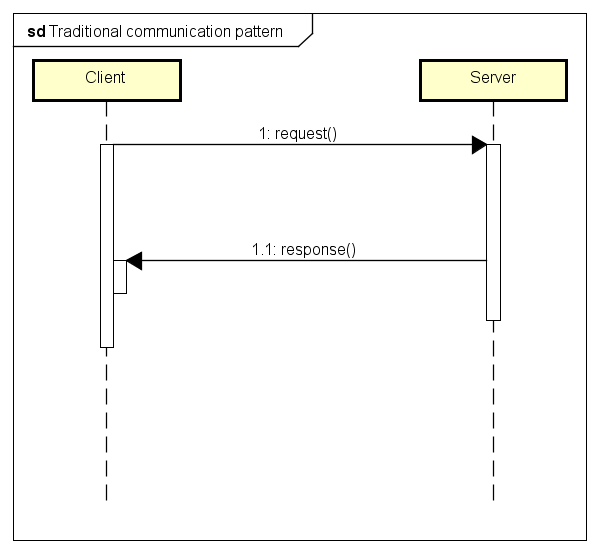
\includegraphics[width=0.68\textwidth]{figures/02_analysis/Traditional-communication-pattern}
    \caption{Traditional client-server communication pattern}
    \label{fig:traditional-communication}
\end{figure}

\begin{figure}[H]
	\centering
	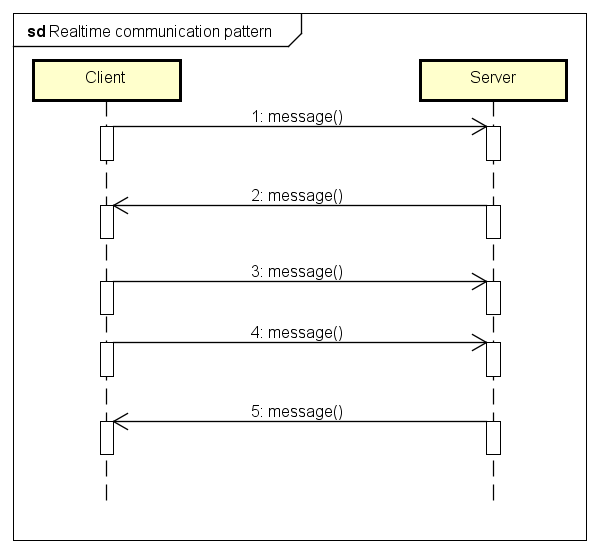
\includegraphics[width=0.68\textwidth]{figures/02_analysis/Realtime-communication-pattern}
    \caption{Realtime client-server communication pattern}
    \label{fig:realtime-communication-pattern}
\end{figure}

While the basic pattern appears simple, the situation quickly begins to complicate once the facts that systems need to deliver realtime data to a large number of devices, often running on different platforms (eg. mobile or web platforms) and that devices may have periods of non-connectivity, such as a mobile device losing reception, are taken into account.

A very simple example of such a situation can be seen in Figure ~\ref{fig:example-situation}. A service needs to send two different messages to two groups of users, that are using different platforms and some of them even have multiple devices at once (eg. a web application in a browser on their computer and a smart phone) and the message needs to be delivered to all of these. For simplicity, only a one way message delivery is illustrated, but for true interactivity such a system must be able to also receive data, not just send it.

\begin{figure}[H]
	\centering
	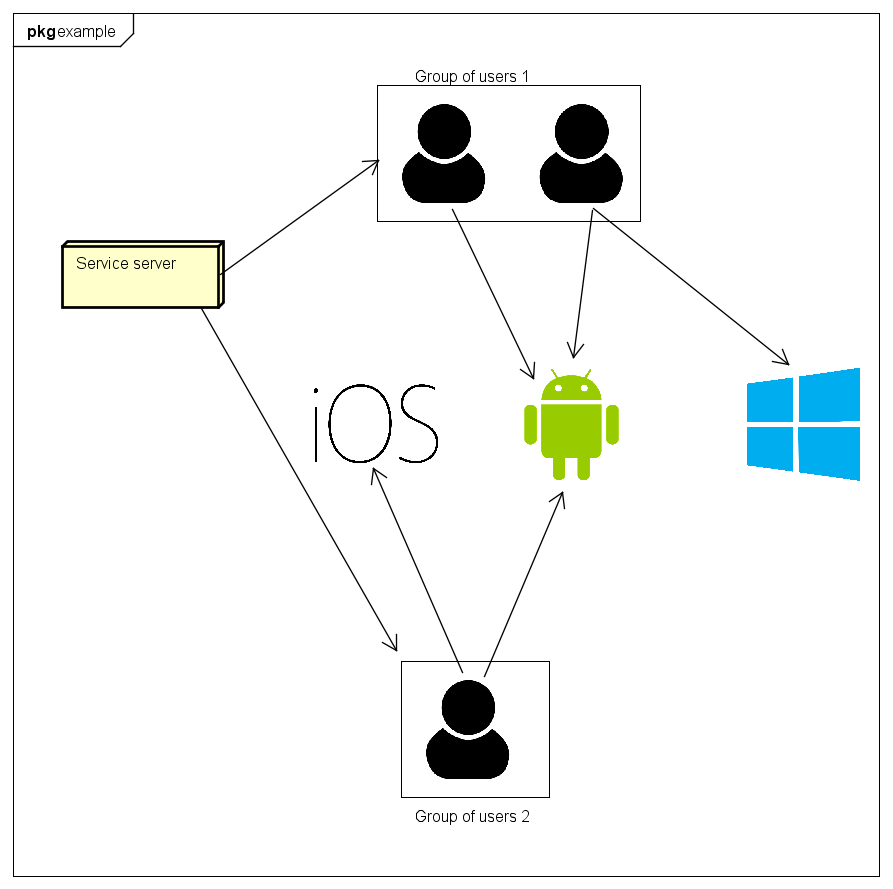
\includegraphics[width=0.8\textwidth]{figures/02_analysis/example-situation}
    \caption{Example situation of message delivery}
    \label{fig:example-situation}
\end{figure}

\section{Existing Similar Solutions} \label{sec:similar-solutions}
At the moment there are several products on the market that provide messaging with differing capabilities and pricing strategies.

Henceforth will be described an overview of some of the most popular ones at the time of writing, based on information provided in marketing materials, documentations and FAQs (Frequently Asked Questions). An in-depth comparison of the inner workings of these is not included, since all of the solutions in question operate on a closed-source basis and do not disclose much information regarding the inner workings of their algorithms and data structures. Furthermore, they are all provided as a service, without a possibility of self-deployment, so a comparison of their performance cannot be made on similar hardware.

\subsection{PubNub}
PubNub\footnote{PubNub <\url{https://www.pubnub.com/}>} is a commercial realtime messaging service based on a Publish-Subscribe pattern. One of the largest messaging service providers in the world, PubNub boasts, among others, secure end-to-end encryption, unlimited number of channels and 250ms latencies worldwide~\protect\cite{pubnub-messaging} and with over 70+ SDKs\footnote{PubNub SDK full list <\url{https://www.pubnub.com/docs}>} can be used on virtually any platform.

\subsubsection*{Key features:}
\begin{itemize}
\item Unlimited Publish/Subscribe channels~\protect\cite{pubnub-messaging} (technically, though device and message amounts are limited with tier-based pricing)
\item 250ms latency worldwide~\protect\cite{pubnub-messaging}
\item Push notification support for Android, iOS and Windows
\item Message delivery once target device comes online (catch-up) as long as message is still in queue. Messages are held in the queue by default for approximately 5 minutes or 100 messages (whichever is reached first), but can be extended using the Storage add-on.~\protect\cite{pubnub-catchup}
\end{itemize}

\subsubsection*{Pricing\footnote{As of January 3 2018} (monthly):}
\begin{itemize}
\item Free: allows 100 daily active devices and 1 million total messages
\item \$49: 500 daily active devices
\item \$149: 1 500 daily active devices
\item \$399: 5 000 daily active devices
\item \$799: 20 000 daily active devices
\end{itemize}

\subsection{Ably}
Ably\footnote{Ably <\url{https://www.ably.io/}>} is a commercial real-time data delivery platform based on a Publish-Subscribe pattern, similarly to PubNub. Apart from several client libraries including ones for Javascript, Java, Python, PHP and others\cite{ably-sdk}, Ably provides WebSocket and REST based APIs~\protect\cite{ably-docs}. Just like PubNub, Ably also provides secure end-to-end encryption.

\subsubsection*{Key features:}
\begin{itemize}
\item Presence awareness, ie. notification when a device becomes online or offline
\item Messages are stored for redelivery for 2 minutes by default. It can however be expanded with the channel message history where messages are stored for up to 24-72 hours~\protect\cite{ably-history} with persisted history enabled.
\item Binary encoded messages help reduce bandwidth and streamlines processing time for encoding and decoding messages~\protect\cite{ably-bin-enc}
\item Message and worker queues
\item Reliable message ordering~\protect\cite{ably-order} - devices are guaranteed to receive messages in the order they were sent
\item WebHooks, which are essentialy HTTP callbacks
\item Simple WebSocket and REST APIs allow for easy client implementation for platforms other than officially supported
\item Protocol adapters providing interoperability between other real-time and queuing protocols~\protect\cite{ably-adapters}
\end{itemize}

\subsubsection*{Pricing\footnote{As of January 3 2018} (monthly):}

Unlike PubNub's tier-based monthly pricing system, Ably provides a more flexible monetization model:
\begin{itemize}
\item Free: 100 peak connections(see Figure ~\ref{fig:peak-conns} ) and channels, 3 million monthly messages
\item Self-service: \$12.50 per thousand peak connections or channels, \$1.25 per million messages. Volume discounts possible
\item Enterprise: tailored package with premium support and no hard limits
\end{itemize}

\subsection{Pusher}
Pusher\footnote{Pusher <\url{https://pusher.com/}>} is a commercial real-time messaging service, also based on a Publish-Subscribe pattern. Pusher provides WebSocket and HTTP APIs for message publishing. Like all previously mentioned services, Pusher also supports end-to-end encryption.

Pusher provides official SDKs for both sending and receiving messages for several languages and frameworks including Go, Java, Node.js, Javascript, Swift, PHP, Python and others\cite{pusher-libs}. 

There is also a range of community developed and maintained libraries including clients for languages and frameworks such as Grails, Flash, ActionScript, Arduino, Haskell and more\cite{pusher-libs2}.

\subsubsection*{Key features:}
\begin{itemize}
\item WebSockets with fallbacks in case they are not available
\item Client events. These include when a device becomes online or offline
\item Android and iOS support
\item Status API for retrieving information such as occupied channels, number of connected devices, etc\cite{pusher-query}
\item Webhooks
\end{itemize}

\subsubsection*{Pricing\footnote{As of January 3 2018} (monthly):}

Pusher offers a tier-based model similar to PubNub

\begin{itemize}
\item Free: 100 peak connections, unlimited channels, 200 000 messages per day (for comparison with Ably, this equals between 5.6 and 6.2 million messages per month, based on the number of days in said month)
\item \$49: 500 peak connections, 1 million messages per day (28-31 million messages per month)
\item \$99: 2 000 peak connections, 4 million messages per day (112-124 million messages per month)
\item \$299: 5 000 peak connections, 10 million messages per day (280-310 million messages per month)
\item \$499: 10 000 peak connections, 20 million messages per day (560-620 million messages per month)
\item Tailored: a custom pricing plan made to fit
\end{itemize}

\subsection{OneSignal}
OneSignal\footnote{OneSignal <\url{https://onesignal.com/}>} is a commercial closed-source high volume push notification delivery service. Compared to PubNub, Ably or Pusher, OneSignal specializes in push notifications for mobile apps, though it does also support web notifications. This fact restricts the amount of platforms OneSignal can be used on in a significant manner.

While all over-the-network communication with OneSignal and then Apple/Android servers is done over HTTPS, compared to the aforementioned services it does not support end-to-end encryption out of the box\cite{onesignal-https}. However, this can be implemented on a server-client basis, ie. encrypt message before sending to OneSignal and then decrypt in app on target device, although this method couldn't be used to send notifications through OneSignal's useful dashboard.

OneSignal provides SDKs for many cross-platform mobile development environments such as Unity, PhoneGap, React Native, Xamarin, and others.

\subsubsection*{Key features~\protect\cite{onesignal}:}
\begin{itemize}
\item A/B Test Messages
\item Scheduled notifications
\item Android, iOS and WebPush notifications support
\item Simple dashboard for managing notifications and users
\item Default time to live for notifications when device is offline is 72 hours\cite{onesignal-ttl}
\item Free
\end{itemize}

\subsubsection*{Pricing:}

Unlike PubNub, Ably or Pusher, OneSignal offers unlimited devices and notifications for free. Its monetization strategy is based on providing premium support.

\subsubsection*{Main feature comparison}

\begin{table}[!ht]
\begin{center}
\begin{tabular}{|l|l|l|l|l|}
\hline
\textbf{Feature} & \textbf{PubNub} & \textbf{Ably} & \textbf{Pusher} & \textbf{OneSignal} \\
\hline
Publish/Subscribe channels & YES & YES & YES & NO \\
\hline
Receive message during short disconnects & YES & YES & NO & YES \\
\hline
Time message is held if device is offline & 5 minutes & 24-72 hours & N/A & 72 hours \\
\hline
End-to-End encryption & YES & YES & YES & NO \\
\hline
Scheduled messages & NO & NO & NO & YES \\
\hline
Device online/offline events & YES & YES & YES & NO \\
\hline
Pricing & Tier based & Usage based & Tier based & Free \\
\hline
Can be self hosted & NO & NO & NO & NO \\
\hline
Open Source & NO & NO & NO & NO \\
\hline
\end{tabular}
\end{center}
\caption{Similar solutions feature comparison}
\label{tab:ex_db}
\end{table}

\begin{figure}[!ht]
	\centering
	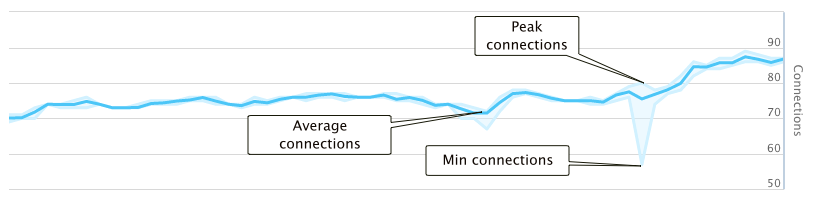
\includegraphics[width=0.8\textwidth]{figures/02_analysis/peak-conns}
    \caption{Peak connections metric. Often used as a metric for pricing messaging services. Source\cite{ably-peak}}
    \label{fig:peak-conns}
\end{figure}

\subsection{Similar solution comparison conclusion}
All four aforementioned provide a service that allows sending a high volume of messages to many connected devices, with a similar list of additional features and different language or framework support and pricing. All have slightly different use cases and offer varying degrees of flexibility and support options.

PubNub, Ably and Pusher provide different restrictions based on the price of their service. Both Ably and Pusher use a peak connections metric, that is defined by the maximum amount of concurrent connected devices (see Figure ~\ref{fig:peak-conns} ). PubNub, on the other hand, has stopped using the peak connection metric\cite{pubnub-peak} in favour of using Daily Active Devices. This metric refers to the total amount of connected devices in a 24-hour period.

However, all of the compared solutions are closed source and provide no means of self hosting. This leads to an intrinsic dependency on the companies that develop and maintain these platforms. This can be a problem for applications using these services if, for example, the pricing was suddenly changed, or the service was shut down entirely. A perfect example of this is when GoInstant was shut down and its customers were forced to switch to a different technology, one of these being PubNub, who offered a guide for migration\cite{pubnub-goinstant}.

\section{Requirement Analysis (Core System)}

After thorough analysis of what is expected of the system, the following requirements are put in place. These requirements are split into two categories, functional and non-functional requirements.

\subsection{Functional Requirements}
Functional requirements define the behaviour of the system.
\begin{itemize}
\item The system must be able to transmit messages between devices
\item The system must be able to deliver a single message to a single device
\item The system must be able to deliver a single message to several devices
\item The system must be able to receive messages from devices
\end{itemize}

\subsection{Non-functional Requirements}
Non-functional requirements define the properties of the system.
\begin{itemize}
\item The server side of the system must be easily horizontally scalable, ie. scaling by adding new instances of the application
\item The server side of the system must be modular, so that methods of receiving and sending messages can be easily replaced or added
\item The server side of the system must be testable
\item The server side of the system must be implemented so that it may run on the JVM\footnote{Java Virtual Machine} platform
\item The system must include a client library for representatives of the following platforms: web, mobile, desktop and server
\item Third party software, such as libraries, used by the system must be open source
\end{itemize}

\section{Requirement Analysis (Sample Implementation)} \label{sec:sample-implementation-analysis}

In order to prove the system meets its requirements and works properly, a sample implementation of the highly modular parts of the system must be provided. This sample implementation must meet the following functional and non-functional requirements:

\subsection{Functional Requirements}\label{sec:s-impl-func-req}
Functional requirements define the behaviour of the system.
\begin{itemize}
\item The sample implementation must be able to deliver notifications and messages onto a mobile platform
\item The sample implementation must be able to deliver notifications and messages onto the Web platform
\item The sample implementation must be able to deliver notifications and messages onto the a desktop platform
\item The sample implementation must be able to deliver notifications and messages onto the a server platform
\item The sample implementation must contain a simple application to showcase the functionality of the system
\end{itemize}

\subsection{Non-functional Requirements}
Non-functional requirements define the properties of the system.
\begin{itemize}
\item The sample implementation must include a module implementing database functionality for a relational database, eg. MySQL, PostgreSQL, MariaDB.
\item The sample implementation must include a module implementing the message queue functionality for a chosen platform, eg. ActiveMQ, RabbitMQ.
\end{itemize}

\section{Platform Analysis}

While the system is designed in such a way that adding or removing supported platforms is simple, for the purposes of this thesis support is to be implemented for representatives of the mobile, web, server and desktop platforms, one each.

\subsection{Mobile platform}
Mobile devices, such as smart phones and tablets are taking over many of the functions that used to be exclusive to desktop computers. With this, it is a growing platform that cannot be overlooked by any modern application.

This section compares the two most popular mobile platforms, Android and iOS, and elaborates on the choice for the mobile platform representative implemented as part of this thesis.

\subsubsection{Android}
Android\footnote{Android <\url{https://www.android.com/}>} is a mobile operating system developed by Google\footnote{Google <\url{https://www.google.com/}>} widely used in smart phones, tablets, televisions, wearables such as smart watches, and even automobiles. With around 80\% market share (see Figure ~\ref{fig:statista-mobile-market}) between mobile operating systems, it is indisputably one of the most important platforms on the market.

While development is lead mostly by Google, Android is an open source project. Its wide adoption by many manufacturers for different purposes is a direct result of this. The Android platform is based on a Linux kernel and apps are run using Android Runtime (ART)\footnote{ART <\url{https://source.android.com/devices/tech/dalvik/}>} created specifically for Android and uses the Dalvik Executable (Dex) bytecode specification.

Development for Android can be done using the Android SDK, which allows the use of Java and Kotlin languages. While ART and the Android SDK closely mimic the Java Runtime Environment (JRE) and Java Development Kit (JDK) respectively, it has some slight differences.

\begin{figure}[!ht]
	\centering
	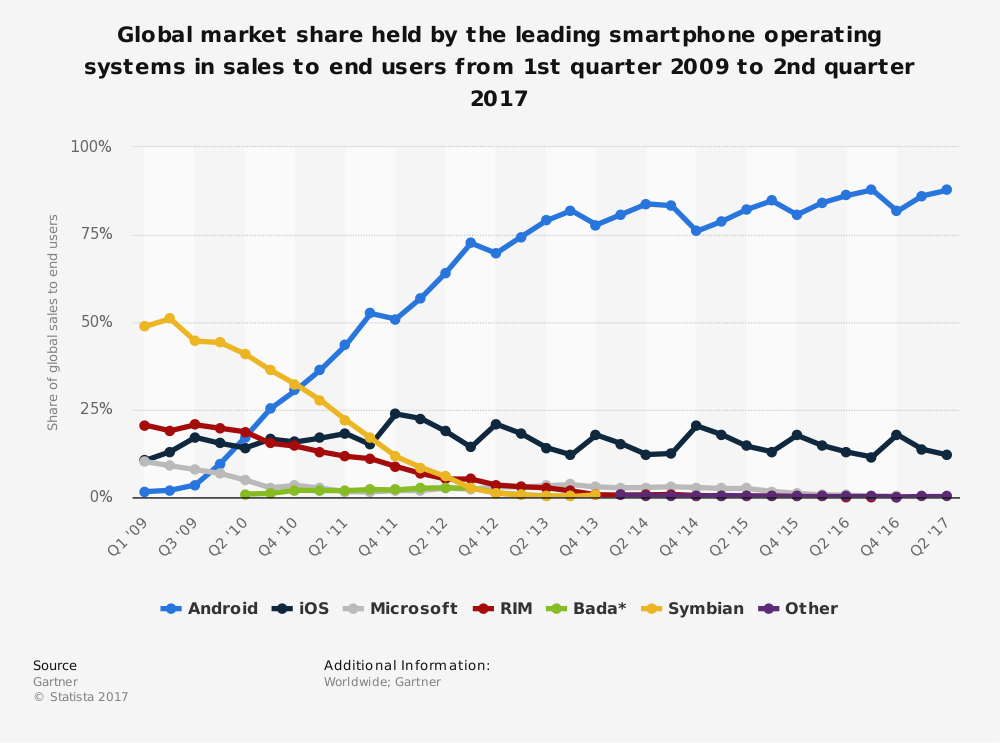
\includegraphics[width=0.8\textwidth]{figures/02_analysis/mobile-market}
    \caption{Global mobile OS market share in sales to end users. Source\cite{statista-mobile-share}}
    \label{fig:statista-mobile-market}
\end{figure}

\subsubsection{iOS}
iOS\footnote{iOS <\url{https://www.apple.com/lae/ios/ios-11/}>} is a mobile operating system developed by Apple\footnote{Apple <\url{https://www.apple.com/}>} used in smart phones, tablets, wearables such as smart watches, and other devices. Unlike Google's Android, iOS is a completely proprietary and closed source platform and can only be found on devices directly developed and sold by Apple. It is the second most popular mobile operating system (see Figure ~\ref{fig:statista-mobile-market}).

Development for iOS can be done using Xcode, Apple’s Integrated Development Environment (IDE). While previously iOS apps were built mostly using Objective-C, Apple has been pushing forward their Swift\footnote{Swift <\url{https://developer.apple.com/swift/}>} language as the future of iOS (and MacOS) app development.

\subsubsection*{Choice of mobile platform for implementation}
The mobile platform chosen for the implementation is Android. Not only does Android possess the majority share of the market, its accessibility and openness to developers is a great advantage. In order to develop an application for Andorid, the developer only needs to download the Android Studio IDE and Android SDK, which are both available for Windows, Mac, and Linux. No physical device is needed for running the application during development, as the SDK contains a powerful emulator. For developing on a physical Android device, the developer can easily turn the device into development mode in the device's settings. 

Developing Android applications and distributing them through own means is completely free. However, most applications are published to Google's official marketplace, Google Play, for which Google has a one time \$25 USD registration fee\cite{google-play-fee}, after which the developer may publish any number of applications on the marketplace.

Developing applications for iOS, however, is much more complicated due to Apple's closed ecosystem. iOS applications may only be developed on Mac devices\cite{apple-dev} and an iOS device is needed to run the application during development. Apple also requires all developers to be enrolled in their Apple Developer Program, which has an annual fee of \$99 USD, or \$299 USD for their Apple Developer Enterprise Program\cite{apple-dev-price}.

\subsection{Desktop and Server platforms}
\subsubsection{Java}
Java\footnote{Java <\url{https://www.java.com/}>} is a popular language owned by Oracle\footnote{Oracle <\url{https://www.oracle.com/}>} that is compiled into Java bytecode, which can be run on any Java Virtual Machine (JVM), regardless of the underlying platform that the JVM is running on. 

Although nowadays it is one of the most popular platforms for developing enterprise server applications, owing to its large community support including extensive libraries, frameworks and platform independence, it can also be used to develop traditional desktop applications, both console based and with a Graphical User Interface (GUI).

\subsection{Web}
Frontend web applications based on HTML, CSS and JavaScript\footnote{HTML <\url{https://www.w3.org/wiki/The_web_standards_model_-_HTML_CSS_and_JavaScript/}>} as more full fledged and interactive applications, compared to the static web sites of the past, have been gaining on popularity. This is partly due to modern browsers and faster internet bandwidths and speeds and partly due to a boom in powerful JavaScript-based frameworks and libraries facilitating the development of extensive, interactive applications that run inside a user's web browser.

A large number of applications have been moving some and in cases even most of their application logic from backend servers to clients in web browsers. In order for these applications to be responsive and interactive, it is key to have real-time reliable communication with any components that are on a remote server.

\section{Analysis of Solutions for Implementation}
In order for the implementation of the core system to meet all of its requirements, a careful and well-informed choice of the proper tools is paramount. This section describes the chosen tools as well as elaborates on the reasons as to why these tools were chosen.
\subsection{Spring Boot}
Spring Boot\footnote{Spring Boot <\url{https://projects.spring.io/spring-boot/}>} is a JVM based framework for creating stand-alone production-grade applications based on the popular Spring Framework\footnote{Spring <\url{https://spring.io/}>}. Unlike most other enterprise Java frameworks, Spring Boot does not need a container (such as Tomcat or Glassfish) to be present on the machine to run in, as it includes an embedded one. This allows for easy and simple JAR (Java ARchive) based deployment.

Spring Boot is an opinionated framework, building on the idea of \textit{Convention over Configuration}. In essence, the idea behind this is to reduce the amount of configuration needed by having sensible defaults and using rules, or conventions, in naming and structure so that the framework may assume, based on these conventions, what it is supposed to do. A typical exam of this would be that a class called \textit{WelcomeController} would map to the \textit{'/welcome*'} URL\cite{convention-over-conf}.

Spring Boot, being based on the Spring Framework, has powerfull Inversion of Control (IoC) capabilites, also known as Dependency Injection (DI). IoC \texttt{"... is a process whereby objects define their dependencies, that is, the other objects they work with, only through constructor arguments, arguments to a factory method, or properties that are set on the object instance after it is constructed or returned from a factory method. The container then injects those dependencies when it creates the bean. This process is fundamentally the inverse, hence the name Inversion of Control (IoC), of the bean itself controlling the instantiation or location of its dependencies by using direct construction of classes, or a mechanism such as the Service Locator pattern."}\cite{ioc}

By delegating the creation and management of objects to the framework, IoC reduces the dependency of components on one another while still allowing them to interact and allows for more modularity, as it is the framework at runtime who decides which instances will be injected, typically by building what is called a Dependency Graph.

Spring Boot projects can be managed by either of the two most popular JVM build automation and dependency management tools, Maven and Gradle.
\subsubsection*{Maven}
Maven\footnote{Apache Maven <\url{https://maven.apache.org/}>} is one of the most popular JVM build automation and dependency management tools. Maven's configuration is based on XML files. It manages the project's dependencies (third-party modules and libraries) and defines the build and execution order of different tasks. Maven also downloads the project's dependencies from online repositories, which are defined in the configuration, and caches them on the local machine.

Maven is distributed as open source under the Apache License, Version 2.0\footnote{Apache License 2.0 <\url{https://www.apache.org/licenses/}>}.

\subsubsection*{Gradle}
Gradle\footnote{Gradle <\url{https://gradle.org/}>} has, over the past few years, become a strong competitor to Maven and gained great popularity\cite{maven-gradle}. Like Maven, Gradle is a build automation and dependency management tool. However, it uses a Groovy-based DSL (Domain-Specific Language) for its configuration. This leads to shorter and more readable configuration files, while at the same time providing more flexibility and even scripting options. Like Maven, Gradle also downloads dependencies from online repositories and stores them on the local machine.

When it comes to performance, thanks to its advanced and modern techniques, Gradle builds are much faster compared to Maven (see Figure ~\ref{fig:maven-gradle-speed}).

\begin{figure}[!ht]
	\centering
	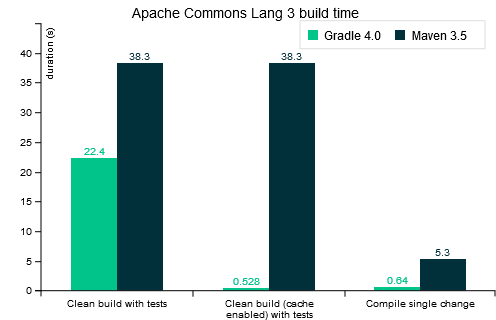
\includegraphics[width=0.8\textwidth]{figures/02_analysis/maven-gradle-speed}
    \caption{Maven and Gradle build time comparison. Source\cite{maven-vs-gradle}}
    \label{fig:maven-gradle-speed}
\end{figure}

Thanks to Gradle's learning curve, ease of use and advanced features, Gradle is the default build tool for Google's Android OS.

Both Gradle and Spring Boot are distributed as Open Source software under the same license as Maven, the Apache License (ASL), Version 2.0 \footnote{Apache License 2.0 <\url{https://www.apache.org/licenses/}>}.

\subsubsection*{Build Tool Conclusion}
After careful evaluation of the available build and dependency management tools, including their features, drawbacks and other factors, such as active community support, extensibility, and thorough documentation among others, the selected tool for the implementation part of this thesis is Gradle.

\subsection{Testing Framework}
In order to create automated tests for the system's code, a powerful testing framework is needed. Automated tests help to ensure that all components work as intended, even after small changes to the underlying code. Testing is indispensable for a large application to remain maintainable.

\subsubsection{JUnit}
JUnit\footnote{JUnit <\url{http://junit.org/junit5/}>} is one of the most popular JVM-based testing framework. Since the JUnit 5 version, it has been split into three main modules, The JUnit Platform, JUnit Jupiter and JUnit Vintage.

The JUnit Platform \texttt{"serves as a foundation for launching testing frameworks on the JVM. It also defines the TestEngine API for developing a testing framework that runs on the platform. Furthermore, the platform provides a Console Launcher to launch the platform from the command line and build plugins for Gradle and Maven as well as a JUnit 4 based Runner for running any TestEngine on the platform."}\cite{junit}

On top of providing the basis for running other testing frameworks, JUnit also provides its own solution for writing tests, which resides in the JUnit Jupiter module.

JUnit is Open Source software released under the Eclipse Public License (EPL) 1.0\footnote{EPL 1.0 <\url{https://opensource.org/licenses/EPL-1.0}>}.

\subsubsection{Spock Framework}
Spock\footnote{Spock Framework <\url{http://spockframework.org/}>} is a powerful all-round testing framework for the JVM platform. Based on the Groovy\footnote{Apache Groovy <\url{http://groovy-lang.org/}>} language and JUnit, it aims to put together the plethora of test libraries available into a comprehensive and easy to use framework. 

Thanks to its use of Groovy DSL, Spock boasts an easy to understand and expressive specification language. On top of basic testing, some of its more advanced features include powerful Mocking APIs, class Stubbing, Data Driven Testing and Interaction Driven Testing, and its Spring Module provides seamless integration with the Spring TestContext Framework\cite{spock}.

Spock Framework is Open Source software distributed under the Apache License (APL) 2.0\footnote{APL 2.0 <\url{https://www.apache.org/licenses/LICENSE-2.0}>}

\subsection{Database technology}
Since the system needs to persistently store, alter and access data, a database system is a proper solution. One of the most commonly used methods of accessing database storage in Java applications is the usage of an ORM (Object-Relational Mapping) framework, arguably the most popular one being Hibernate\footnote{Hibernate <\url{http://hibernate.org/}>}.

Hibernate provides abstraction from the concrete database implementation, along with its own query language, HQL (Hibernate Query Language), which allows for more flexibility and interchangeability when it comes to the database software in use. Hibernate's ORM implementation is also an implementation of the Java Persistence API (JPA)\cite{hibernate-orm}.

On top of powerful ORM for SQL databases, Hibernate also provides Hibernate OGM, a powerful JPA implementation for NoSQL database systems, including first party implementations for Infinispan, MongoDB and Neo4j and community-maintained dialects for Cassandra, CouchDB, EhCache, Apache Ignite and Redis\cite{hibernate-ogm}.

Hibernate is Free Software distributed under the GNU Lesser General Public License (LGPL) 2.1\footnote{LGPL 2.1 <\url{https://www.gnu.org/licenses/old-licenses/lgpl-2.1.html/}>} or Apache License (ASL), Version 2.0\footnote{ASL 2.0 <\url{https://www.apache.org/licenses/LICENSE-2.0.html/}>} licenses.

The aim of the system implemented as part of this thesis is to provide as much freedom, flexibility and modularity to the its users\footnote{Users here meaning those who would self-host the system, not the end users of any application using the system}. For this reason, the system should be designed in such a way that it is easy to switch out the end database layer, including support for both SQL and NoSQL databases, and create custom implementations.

\section{Analysis of Solutions for Sample Implementation}
In order to prove the system meets its requirements and works properly, a sample implementation of the highly modular parts of the system must be provided. The requirements for the sample implementation are listed in Section \ref{sec:sample-implementation-analysis} \nameref{sec:sample-implementation-analysis}.

\subsection{Firebase Cloud Messaging}
Firebase Cloud Messaging (FCM)\footnote{FCM <\url{https://firebase.google.com/docs/cloud-messaging/}>} is a multi-platform messaging solution by Google\footnote{Google <\url{https://google.com}>}. FCM is the successor to the Google Cloud Messaging (GCM)\footnote{GCM <\url{https://developers.google.com/cloud-messaging/}>} platform, that was aimed mainly at the Android, iOS, and Google Chrome platforms. On top of the platform support of GCM, FCM adds support for the Web, NodeJS, C++, and Unity platforms. 

FCM also provides powerful HTTP and XMPP (Extensible Messaging and Presence Protocol) APIs, which can be used to create clients for other platforms.

\subsubsection*{Key Features\cite{fcm}}
\begin{itemize}
\item Support for Android, iOS, Web, C++ and Unity platforms.
\item Unlimited number of messages, with up to 4kB of data each.
\item Support for Notification messages, which display a notification on the target device to the user.
\item Support for Data messages, which are only handled in the background of the app on the target device.
\item Normal and High priority message setting.
\item Message Time to Live (TTL).
\item HTTP and XMPP APIs.
\item Free of charge.
\end{itemize}

Firebase Cloud Messaging is used in the sample implementation to relay messages onto the Android platform.

In order to simplify the use of FCM from the system a proper client library should be used. While there are no first party Java libraries, there are several community-maintained ones, two of which are compared below.

\subsubsection{FcmJava}
FcmJava\footnote{FcmJava <\url{https://github.com/bytefish/FcmJava}>} is a community-maintained Java library for communication with the FCM API. It provides object-oriented encapsulation of the FCM APIs. At the time of selecting the tools for the sample implementation (14. 1. 2018), FcmJava does not support the new FCM HTTP v1 API, but uses the Legacy HTTP Cloud Messaging, however support for the FCM HTTP v1 API is planned in the 3.0 milestone\cite{fcmJava}.

\subsubsection{Pushraven}
Pushraven\footnote{Pushraven <\url{https://github.com/Raudius/Pushraven}>} is a community-maintained Java library for communicating with the FCM API. It provides a nicely designed object-oriented encapsulation of the FCM APIs, that is simple to use and very easy to read. On 1. 12. 2017, the main auther of Pushraven, Raudius, released a fully updated version of the library with support of the new FCM HTTP v1 API\cite{pushraven-new-api}.

\subsubsection*{FCM library conclusion}
Due to its good design, ease of use, fast update intervals and support of the more modern FCM HTTP v1 APIs, the library used in the sample implementation was decided to be Pushraven.

\subsection{Message Queue}
The design of the architecture of the system features a message queue for passing messages between the individual instances of the application (see Chapter \ref{design:design} \nameref{design:design}). This section presents several of the most popular message queue brokers, discusses their differences and presents a choice for the sample implementation.

\subsubsection{RabbitMQ}
RabbitMQ \footnote{RabbitMQ <\url{https://www.rabbitmq.com/}>} is an Open Source message queue broker, licensed under the Mozzila Public License (MPL)\footnote{MPL <\url{https://www.mozilla.org/en-US/MPL/}>}. RabbitMQ supports deployment in a distributed cluster, allowing for easy scaling, can be deployed on a wide variety of systems including Windows and Linux, and provides client libraries for languages such as Java, .NET, PHP, Python, Javascript, Ruby, Go and others\cite{rabbitmq-devtools}, as well as integration with frameworks such as Spring.

While RabbitMQ is not a JMS provider, it includes a plugin that enables support for the JMS queue and topic messaging models\cite{rabbitmq-jms}.

\subsubsection*{Key features:}
\begin{itemize}
\item Support for both message queues and publish/subscribe pattern topics
\item Delivery acknowledgement
\item Routing based on wildcards
\end{itemize}

\subsubsection{Apache ActiveMQ}
Apache ActiveMQ \footnote{Apache ActiveMQ <\url{http://activemq.apache.org/}>} is an Open Source message queue broker, licensed under the Apache 2.0 License (APLv2)\footnote{APLv2 <\url{http://www.apache.org/licenses/LICENSE-2.0.html}>}. ActiveMQ provides a plethora of clients and protocols for languages such as Java, C++, C\#, Ruby, Perl, Python, PHP, and others\cite{activemq-devtools}, as well as several different communication protocols, such as AMQP, MQTT, OpenWire and STOMP\cite{activemq-devtools}. ActiveMQ also has support for frameworks such as Spring and unlike RabbitMQ is a JMS provider.

ActiveMQ also provides message queue data persistence and scaling via distribution and clustering.

\subsubsection*{Key features:}
\begin{itemize}
\item Support for both message queues and publish/subscribe pattern topics
\item Delivery acknowledgement
\item Routing based on wildcards
\end{itemize}

\subsubsection*{Message Queue broker conclusion}
RabbitMQ and Apache ActiveMQ provide extremely similar functionality and therefore are equivalent solutions for the implemention. However, based on the fact that ActiveMQ itself is based on the JVM and is a native JMS provider, as well as prior personal experience with the platform, the message queue broker used in the implementation is Apache ActiveMQ.

\section{Scalability Analysis}
In order to achieve a system that is horizontally scalable, the system must be able to easily run distributed among different machines, let us call every such instance of the back-end application a \textit{node}. The system must be able to run across multiple nodes, distributing the computational load among these and it must be easy to add or remove nodes from the system while it maintains full functionality. This section describes the requirements on such a system and various problematic scenarios that may occur and the system must be able to handle.

\subsection{Problematic Scenarios} \label{analysis-scale}
\subsubsection{Servicing a large amount of clients} \label{analysis-scale-large-no}
This is the most basic use case for a scalable system. The system must be able to service a large amount of clients at the same time without any significant performance loss or becoming overloaded and stop servicing them at all.

This is a problematic scenario for applications as the infrastructure an application runs on has limited resources. An increasing amount of clients can be serviced by vertically scaling the application, i.e. adding more resources, such as CPU speed and/or cores and RAM memory, but this approach is feasible only to some extent, which is where horizontal scaling comes into play. By scaling the system horizontally, onto multiple machines, the load can be better distributed.

This scenario is expected to appear very often, as a large amount of clients are to be using the system simultaneously.

\subsubsection{A large amount of clients connects at the same time}
This scenario may occur when a large amount of clients attempts to connect to the system simultaneously. The difference between this scenario and the scenario described in Section \ref{analysis-scale-large-no} \nameref{analysis-scale-large-no} is that a large number of clients must not only be serviced at the same time, but they are also initializing their connection to the system simultaneously, placing great strain onto the entry point of the system.

This scenario is expected to occur very rarely on a very large scale and in minor scales during peak times, for example if an application utilizing the system would connect when the user starts using their phone a peak of connections can be expected in the morning, when people wake up and start their day.

\subsubsection{A large amount of messages for a single client}
This case describes a scenario where a large number of clients are all sending messages to a single addressee client. The possible problem is that a client is connected to a single node, therefore the messages that are to be delivered to it cannot be scaled across multiple nodes.

This scenario may happen in cases where the system is used to link a server to its clients, for example let us imagine a tracking app for food delivery. The individual clients would be the apps on the phones of each delivery driver, while the client receiving all their messages would be the server running the tracking application. All the drivers constantly stream their position data to the "server" through the system, resulting in a large number of messages from various clients, all addressed to a single recipient client.

\subsubsection{A node dies}
This scenario describes a situation where one of the nodes dies or is disconnected. The system must be able to respond to such a situation by reconnecting any clients that were connected to this node to a different node or set of nodes and manage to reroute any messages that are addressed to these clients.

This scenario is expected to happen rarely, with a cause either due to technical issues or for example upgrading the application on a node to a new version.

\subsubsection{A message is sent to a user group with a large amount of users}
This scenario describes a situation where the system contains a group with many users, for example an application's group of all its users, and a message is sent to this group. In the aforementioned example that could be used as a broadcast message to all the app's users. This scenario is problematic as the number of users in the group may be large enough that unfolding the group into all its users may put extreme stress on a node and its memory, possibly causing it to crash.

This scenario is expected to occur depending on the application using the system.

\chapter{Design}
This chapter provides an in-depth description of the system architecture and its individual components, based heavily on the conclusions drawn from Chapter \ref{chap:analysis} \nameref{chap:analysis}.

\section{Architecture Design}
The system can be divided into multiple main parts\footnote{Note: These do not necessarily overlap with the modular aspects of the system.}, the highest-level of division can be into a basic  three-layered architecture containing these three layers:
\begin{itemize}
\item Client layer
\item Business layer
\item Data layer (often referred to as Storage layer)
\end{itemize}

Figure ~\ref{fig:layer-arch} shows these three layers and the components belonging in each. Due to the high modularity requirements of the system, only most of the Business layer belongs into the core system, the Client and Data layers are to be easily interchangeable and therefore will be part of the sample implementation. A more concrete version of the tiered architecture for the full sample implementation can be seen in Figure ~\ref{fig:s-impl-arch}.

\begin{figure}[H]
	\centering
	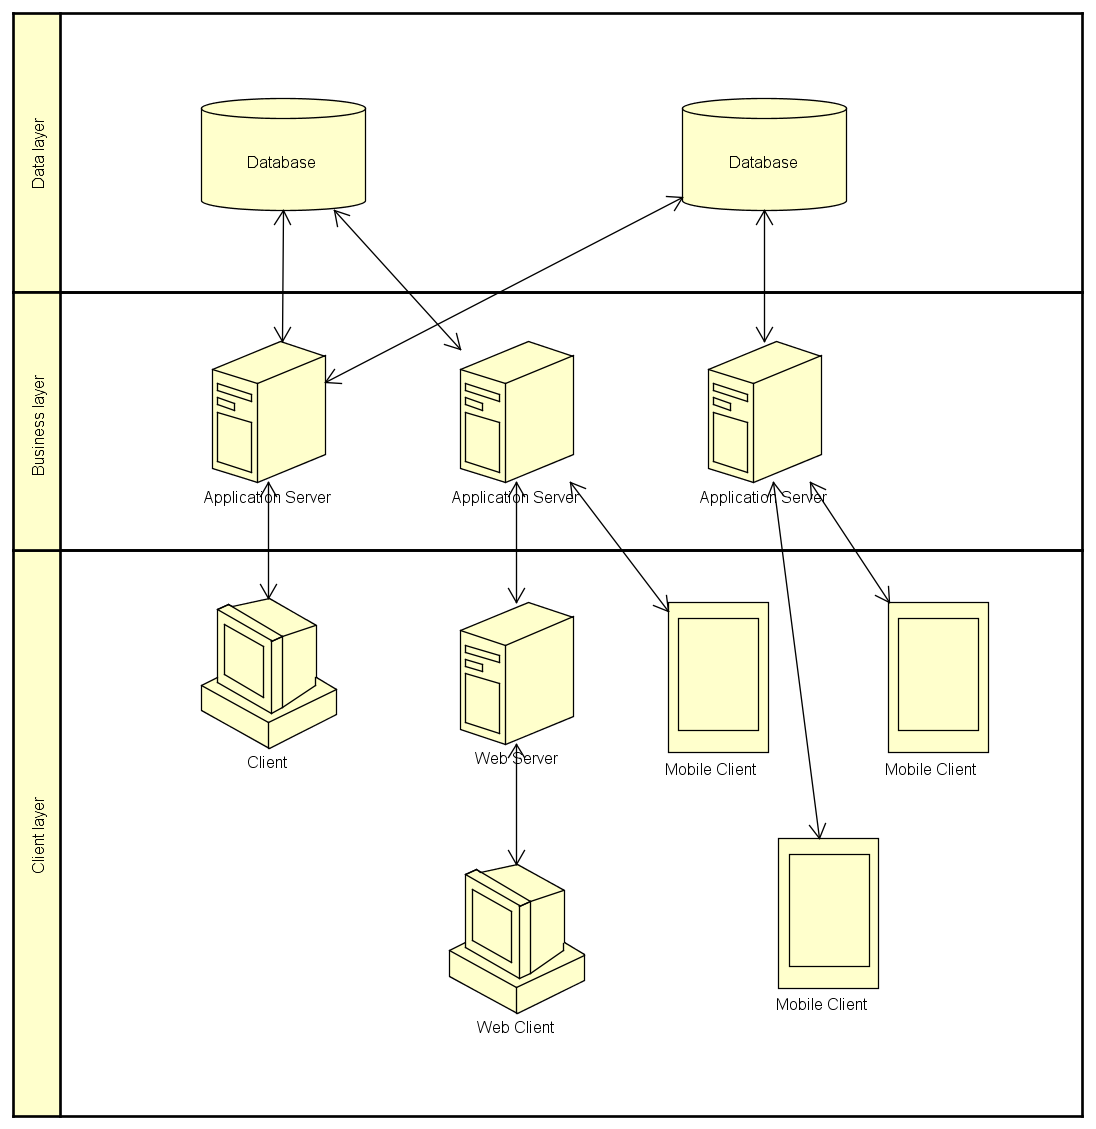
\includegraphics[width=1\textwidth]{figures/03_design/layer-arch}
    \caption{Three layered basic system architecture}
    \label{fig:layer-arch}
\end{figure}

\begin{figure}[H]
	\centering
	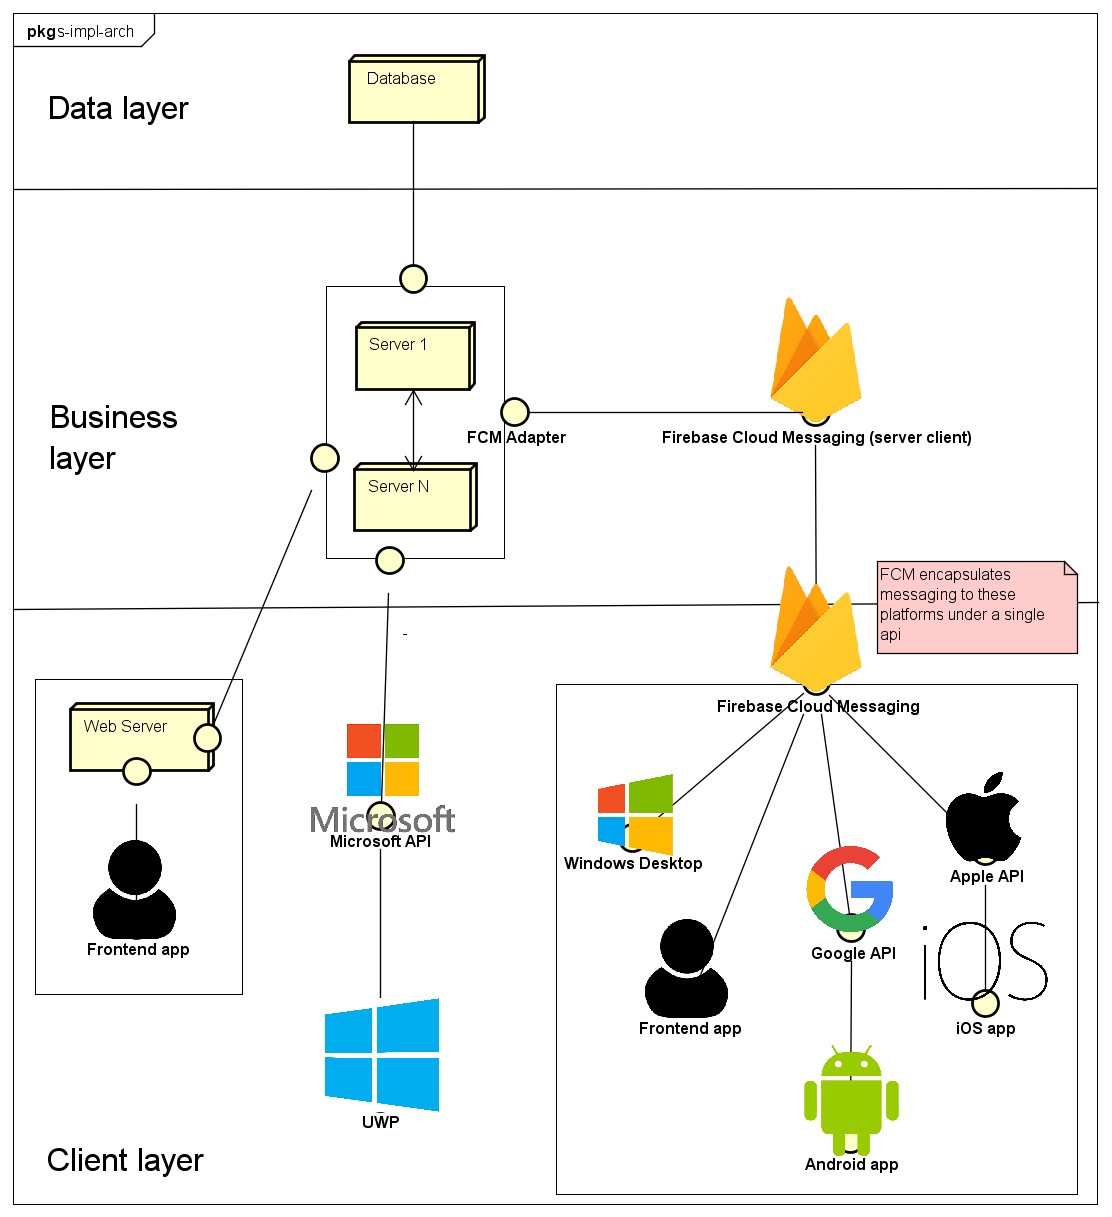
\includegraphics[width=1\textwidth]{figures/03_design/s-impl-arch}
    \caption{Three layered system architecture for sample implementation}
    \label{fig:s-impl-arch}
\end{figure}

\subsection{Data Layer} \label{design:data-layer}
The data layer will be used to persistently store data regarding how messages should be handled and how they are to be delivered to their intended recipient. After analysing the necessary requirements, the data to be stored was divided into the following entities.
\begin{itemize}
\item \textbf{Group:} The Group entity represents a collection of Users, aggregated for some reason, eg. a topic in a publish/subscribe pattern.
\item \textbf{User:} The User entity represents an end user of the application using the system. A User can belong to Groups and has Devices.
\item \textbf{Device:} The Device entity represents an end device onto which messages will be delivered. Every Device belongs to a User and is on a certain Platform.
\item \textbf{Platform:} The Platform entity represents the platform on which a Device is running and therefore determines how a message is to be delivered to that Device, eg. Android, iOS, FCM, etc.
\end{itemize}

Due to the high modularity design required of the system, the core of the system will only contain interfaces and instructions for the implementation of a data layer.

\subsubsection{Sample Implementation Data Layer}
In the sample implementation, which is part of this thesis, a relational database system will be used. The Object-Relational Mapping (ORM) implementation design of the data layer interface can be seen in Figure ~\ref{fig:orm}

\begin{figure}[H]
	\centering
	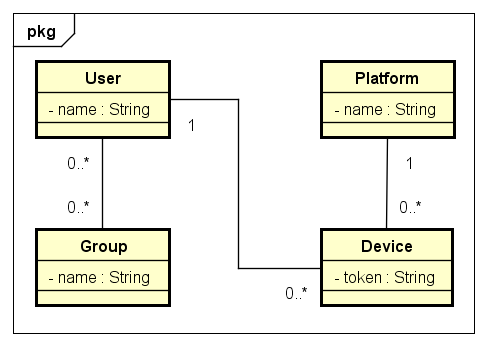
\includegraphics[width=0.6\textwidth]{figures/03_design/orm}
    \caption{Sample Implementation ORM Data Layer design}
    \label{fig:orm}
\end{figure}

\subsection{Business Layer}
The business layer, also commonly known as the business logic layer, is where all the main functions of the system are done. In this case, it is where messages are sorted received, sorted and passed along to their respective adapters\footnote{More on adapters in Section \ref{sec:adapters}} to be sent to their target end devices. 

Figure ~\ref{fig:msg-flow} shows a simplified representation of the flow of a message through the business layer. The message starts at the point from where it is sent, after being received through the system's API it is processed and passed to the MessagingService, which communicated with the Data layer to find information on the groups, users, devices and platforms the message is to be sent to. After this, the message is passed the AdapterService, which then delegates it to the respective adapters of the devices it is meant to be sent to and finally, the message is sent out to the end devices.

\begin{figure}[H]
	\centering
	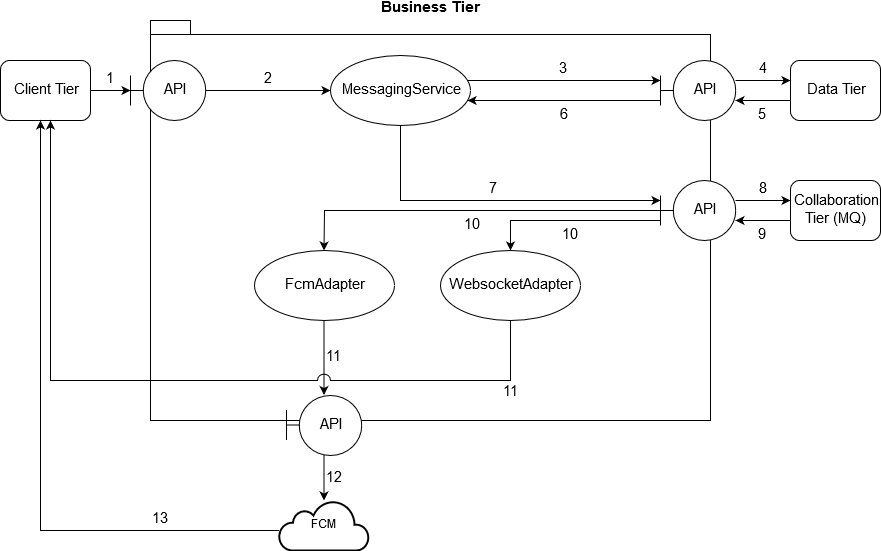
\includegraphics[width=0.8\textwidth]{figures/03_design/msg-flow}
    \caption{Flow of a message through the Business layer}
    \label{fig:msg-flow}
\end{figure}

\subsection{Client Layer}
The client layer includes all client libraries and applications that can receive and/or send messages from/to the system. Because the client layer must be designed with high modularity in mind, none of it is part of the main system and the specifics of its API depend on the individual adapters\footnote{More on adapters in Section \ref{sec:adapters}} that go with it.

\subsubsection{Sample Implementation Client Layer}
The sample implementation that is part of this thesis will include an implementation of the client layer, aka the client libraries, for the platforms stated in Section \ref{sec:s-impl-func-req} \nameref{sec:s-impl-func-req}.
\subsubsection*{Java}
The client library for the Java platform will be a Java Archive (JAR) file, that can be included in a Java application's classpath and provides interfaces to send and receive messages to and from the system, respectively. It will be independent of any framework, such as Spring, so that it works with any Java application.

With real-time communication in mind, the design of the client library was made using an Event Driven architectural pattern. Figure \ref{fig:java-client-classes} shows an overview of the classes the library will contain. The most important class being \textit{MsgrClient}, which is the main point of interaction for the user. It contains methods for sending messages and adding or removing message listeners. Message listeners will be user created implementations of the \textit{IMessageListener} interface. Data container classes are not important to the overall architecture design, they serve simply as POJOs (Plain Old Java Objects) that envelop data, along with providing getters and setters, in order to pass the data between components in a simple, encapsulated object-oriented manner. These include classes such as \textit{Message}, \textit{User}, etc.

\begin{figure}[H]
	\centering
	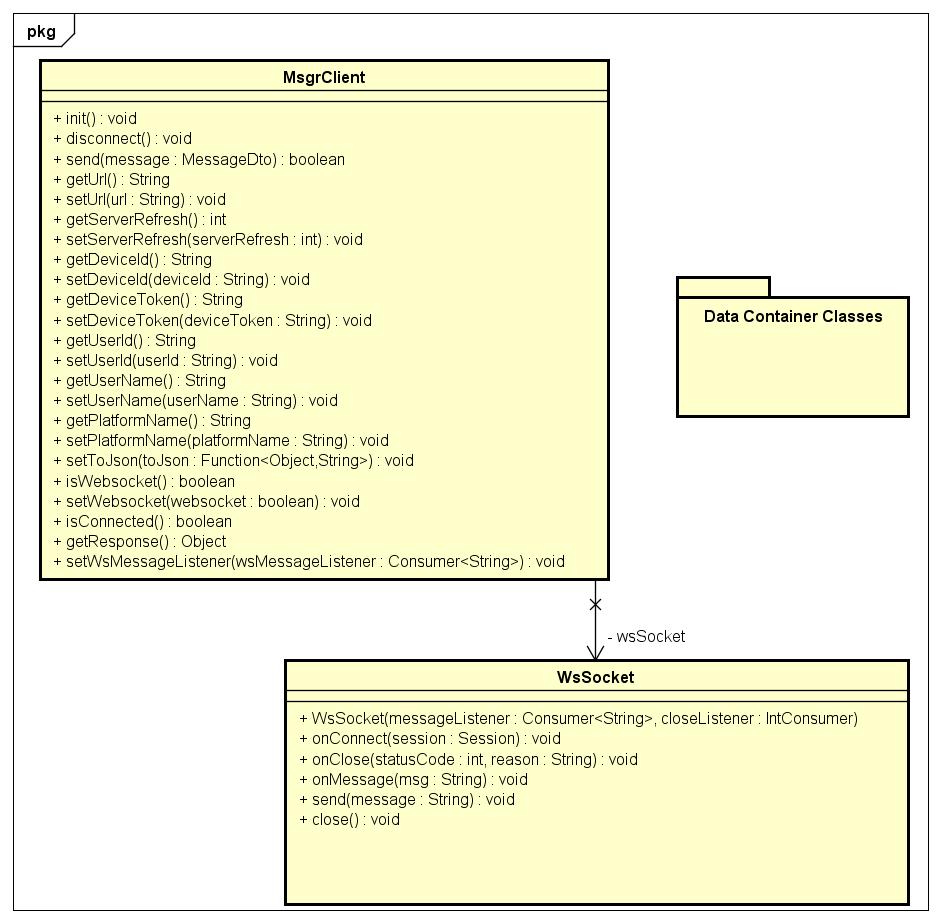
\includegraphics[width=0.8\textwidth]{figures/03_design/java-client-classes}
    \caption{Design of the main class components of the Java client library}
    \label{fig:java-client-classes}
\end{figure}

\subsubsection*{Android \& iOS}
The Android and iOS clients will be simple applications for each platform, using Google's Firebase Cloud Messaging (FCM) client libraries, which are provided for both the Android\cite{fcm-android-client} and iOS\cite{fcm-ios-client} platforms.

\subsubsection*{Web}
The Web client will be a simple HTML, CSS and Javascript application using Google's FCM Javascript client library, which supports the majority of modern browsers (versions: Chrome 50+, Firefox 44+, Opera Mobile 37+)\cite{fcm-web-client}.

\section{Modularity Design}

A critical part of the requirements put onto the system is its high flexibility and adaptability, based on high modularity. For this reason, the system has been designed with maximum modularity in mind. In order to achieve this, the main system is contained in a Core module, which will be the basis for any full applications with the system. Functionality and components that may be interchanged depending on the applications' needs will be contained in modules, which will be added to the full application as further dependencies (side-to-side with the Core module). An example of an application with different modules can be seen in Figure \ref{fig:s-impl-comps}, which shows the module structure that will be used in the Sample Implementation.

\begin{figure}[H]
	\centering
	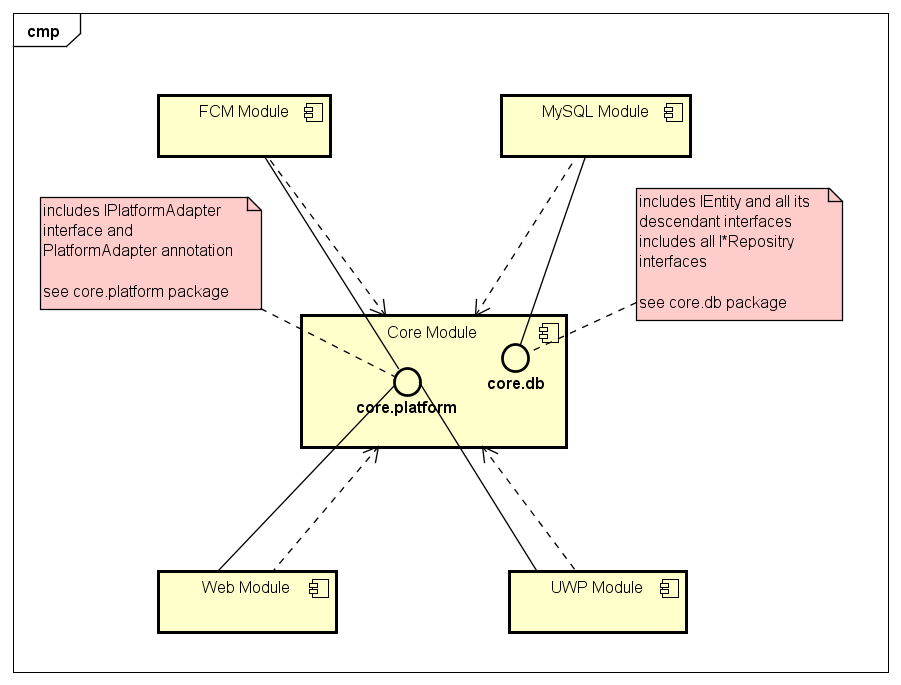
\includegraphics[width=0.8\textwidth]{figures/03_design/s-impl-comps}
    \caption{Module structure design of sample implementation}
    \label{fig:s-impl-comps}
\end{figure}

\subsection{Core Module}
The Core module, or Core library, is the heart of the entire system. The Core module provides the interfaces needed for other modules to implement and Spring Managed Beans (from now on referred to simply as Beans). Beans are objects whose lifecycle is managed by the Spring's IoC Container's Application Context, which means the Spring Container initializes and configures them and where needed, allows them to be injected\cite{spring-beans}. These Beans provide the main business logic of the application as well as manage the cooperation between all modules. The design of these interactions is further elaborated upon in the following sections.

\subsection{Database Modularity} \label{design:database-modularity}
The system's access to the data layer has been designed in a fully modular way, so that the end deployment is not dependent on any one type or provider of database. The result of this effort for maximum freedom and interchangeability are the interfaces in the \textit{core.db} package, as seen in Figure \ref{fig:core-db-module}.

\begin{figure}[!ht]
	\centering
	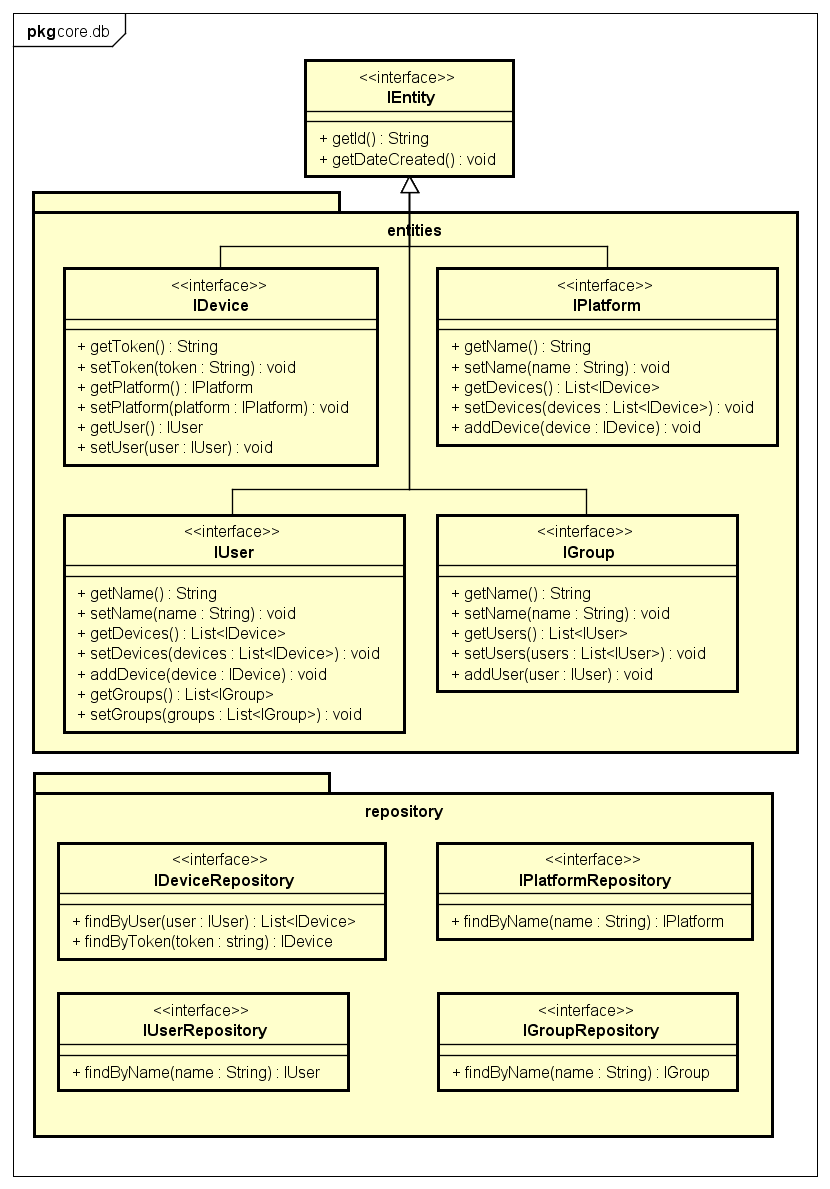
\includegraphics[width=0.95\textwidth]{figures/03_design/core-db-module}
    \caption{Interfaces for database modules in the \textit{core.db} package}
    \label{fig:core-db-module}
\end{figure}

Any module that wishes to implement access to a database must create JPA Entities implementing the entity interfaces and create interfaces that extend the repository interfaces and extend Spring Data's \textit{CrudRepository} interface. This will indicate to the Spring Context to instantiate repository Beans based on these interfaces\cite{spring-repos}, which the Context will then inject into the Beans where they are used.

\subsection{Platform Modularity}
One of the key features of the system is its multi-platform support. In order to be able to support the widest possible range of platforms, the platform portion of the system had to be designed with complete modularity in mind. The results of the design choices made based on these requirements led to the creation of the \textit{IPlatformAdapter} interface and \textit{@PlatformAdapter} annotations, which can be seen in more detail in Figure \ref{fig:core-platform-module}.

\begin{figure}[!htb]
	\centering
	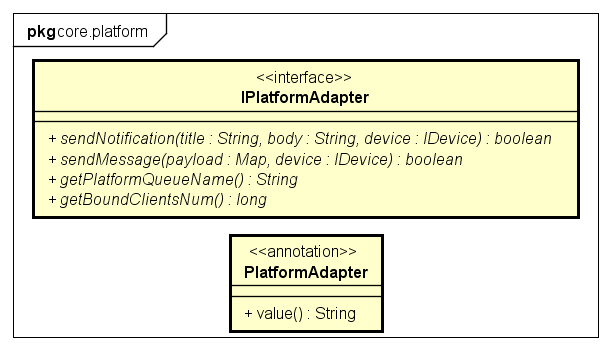
\includegraphics[width=0.95\textwidth]{figures/03_design/core-platform-module}
    \caption{Interfaces for platform modules in the \textit{core.platform} package}
    \label{fig:core-platform-module}
\end{figure}

Any module that wishes to implement support for a new platform must contain at least one Bean implementing the \textit{IPlatformAdapter} interface and annotate it with the \textit{@PlatformAdapter} annotation, which takes the platform's name as a parameter.

\subsubsection{Adapters}\label{sec:adapters}
Platform Adapters are Spring Managed Beans that implement the Core module's \textit{IPlatformAdapter} interface and are annotated with the \textit{@PlatformAdapter} annotation, which takes the platform's name as a parameter. 

Adapters will be automatically found at system startup by the Core module's \textit{AdapterService} using Spring's Application Context and registered based on the platform's name, as specified in the \textit{@PlatformAdapter} annotation. After which whenever a message is sent to a device through the \textit{MessagingService}, the \textit{AdapterService} will provide the Adapter needed to send message for the platform of that device to the \textit{MessagingService}, which will then use it to send the message. The sequence of these events including an example message being sent can be seen illustrated in Figure \ref{fig:adapter-flow}

\begin{figure}[!htb]
	\centering
	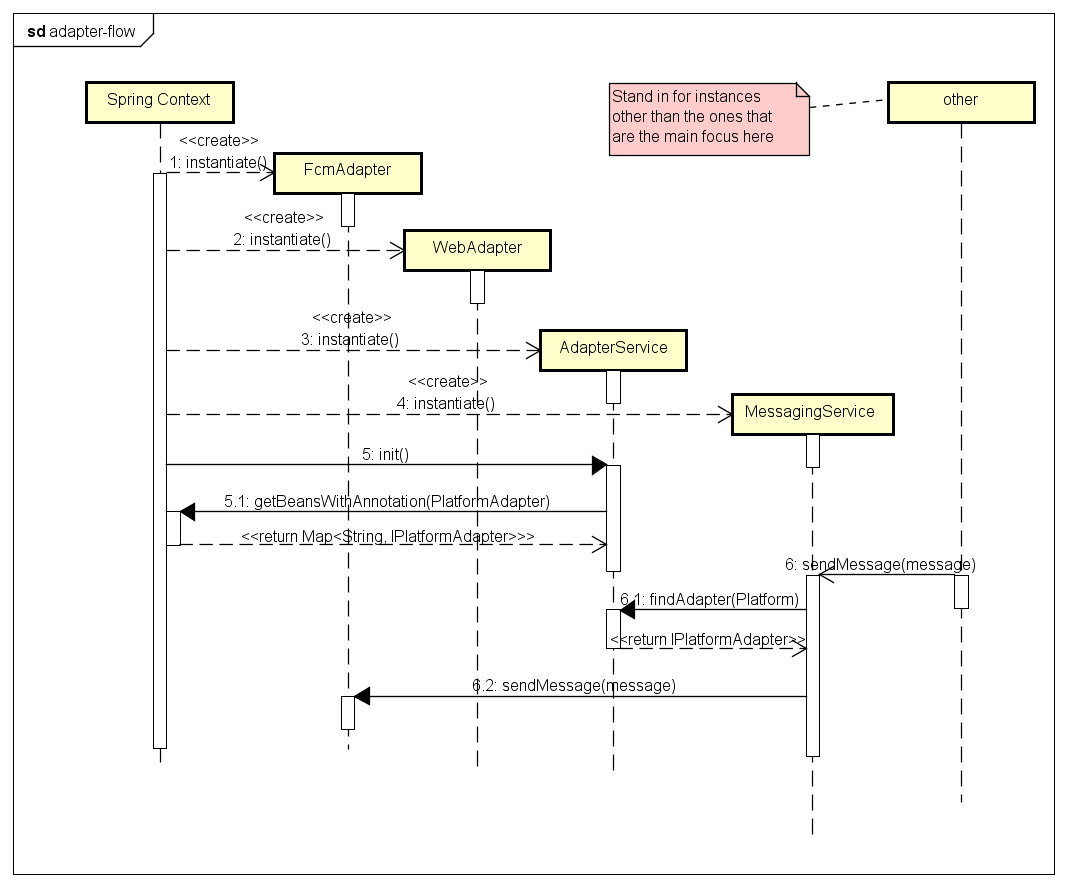
\includegraphics[width=0.9\textwidth]{figures/03_design/adapter-flow}
    \caption{Sequence diagram indicating the resolution process of Adapters}
    \label{fig:adapter-flow}
\end{figure}

\clearpage

\section{Scalability Design}
This section describes the architecture proposed in order to achieve a horizontally scalable system, as well as how the proposed architecture deals with possible problematic scenarios described in Section \ref{analysis-scale} \nameref{analysis-scale}.

The proposed design of the system architecture to achieve horizontal scalability is shown below in Figure \ref{fig:scalability-architecture}. The design can be split into four main components: \textbf{Nodes, Node Coordinator, Message Queue} and \textbf{Database}, the connections between these are shown in the Figure in different colours (see legend in Figure \ref{fig:scalability-architecture}). The responsibilities as well as the way in which the different components are connected and communicate with each other are described in detailed in the following sections.

\begin{figure}[!ht]
	\centering
	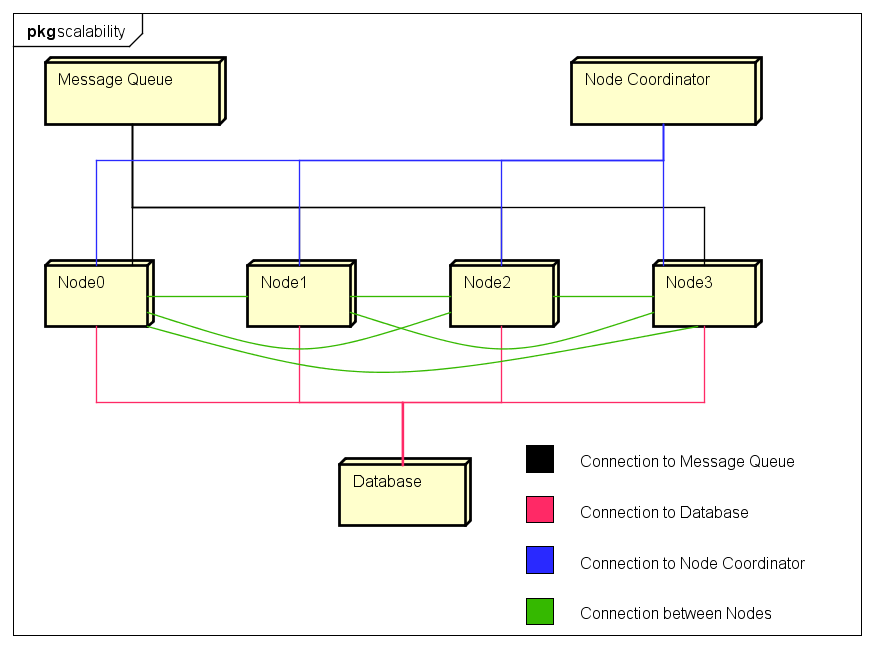
\includegraphics[width=0.9\textwidth]{figures/03_design/scalability-architecture}
    \caption{Architecture design for horizontal scalability}
    \label{fig:scalability-architecture}
\end{figure}

\subsection{Scalability Architecture Components}
\subsubsection{Nodes}
The Nodes form the core of the system. A node is an instance of the application containing all of the business logic. A Node's main responsibility is to dispatch messages to client devices as well as resolving groupings (such as \textit{Group} or \textit{User}, see Section \ref{design:data-layer} \nameref{design:data-layer}). The Nodes are also the system's main scalability point, as the amount of load the system can process is proportional to the number of active Nodes in the system.

Nodes are aware of each other, as they receive a list of Nodes ordered by least load by the Node Coordinator (see Section \ref{design:node-coordinator} \nameref{design:node-coordinator}).

\subsubsection{Node Coordinator} \label{design:node-coordinator}
The Node Coordinator is a simple component, whose main responsibility is to keep track of all Nodes in the system, as well as perform periodical health checks on them. Each Node should connect and announce its presence to the Node Coordinator upon start-up. The Node Coordinator also provides its connected Nodes with a list of \textit{n} least loaded Nodes.

\subsubsection{Message Queue}
The Message Queue component is an implementation of a message queue which is inherently scalable. The message queue channels correspond to individual devices connected to Nodes, i.e. channel \textit{device1} will contain messages addressed to a device with id \textit{device1}, or groupings, i.e. channels \textit{group3} or \textit{user42} for Groups or Users, respectively.

\subsubsection{Database}
The Database component is a database layer shared between Nodes, containing all persistent data. As the database layer is fully modular, the end implementation used is up to the discretion of whoever is building the system (see Section \ref{design:database-modularity} \nameref{design:database-modularity}). However, in order to create a system that is fully scalable a scalable database solution (e.g. database cluster) is recommended.

\chapter{Implementation}

\section{Deployment}

The whole solution is designed for and deployed in the Amazon Web Services (= AWS) cloud environment. It is a managed Virtual Private Cloud (= VPC) environment that is only accessible with company credentials and certificates.

\begin{figure}[!ht]
	\centering
	\includegraphics[width=0.8\textwidth]{figures/04_implementation/deployment_diagram}
    \caption{AWS System Architecture}
\end{figure}

\section{Issue Tracker}

The Issue Tracker used in my work environment is JIRA\footnote{No abbreviation here. It is short for GOJIRA, which is Godzilla in Japanese. Rumor has it that it was called this because the main competing product is Bugzilla.} by Atlassian. It is a standard project management tool providing bug tracking, issue tracking and many other functions. It is conveniently synergistic with other Atlassian tools such as Confluence (for documentation and wiki) and Bitbucket (formerly Stash), which is a server for version control (Mercurial and Git). The advantage is that all these three components are deployed in the AWS VPC environment. Thus, as a programmer, I have fairly easy access to its internal APIs without being afraid to leak data by mistake.

\subsection{API}

JIRA REST API is quite a mess, because Atlassian didn't develop all their products from scratch (Bitbucket was acquired) and it is still visible that the usage isn't seamless. In order to access Teams, Projects and Issues, two API endpoints have to be used:

\begin{enumerate}
	\item JIRA REST API
	\item JIRA REST AGILE
\end{enumerate}

Both of them are APIs (= Application Programming Interface), but I will use their names to distinguish between them. They are similar, but also slightly different from each other. 

To illustrate the subtle differences that drive any software engineer mad:

\begin{itemize}
	\item When JIRA REST API is used to obtain the issues, the resulting array uses pagination, because there could be a lot of issues and loading them all at once could take a significant amount of time. In order to determine whether the array I have is final, a parameter "total" is present in the response. This parameter shows how many issues there are in total. In order to load the whole list, it is necessary to keep track how many there are, and how many are left on the stack.
	
	\item When JIRA REST AGILE is used to obtain the teams, the resulting array also uses pagination. In order to determine whether the array I have is final, a parameter called "isLast" is present in the response, which has, surprisingly, a boolean value true/false. Obviously, when the value is false, one has to load the next page with the last index that came before.
\end{itemize}

There are plenty of these little surprises that are completely fragile with any update of the whole system. I honestly do not know why it isn't the top priority for Atlassian to unite their APIs.

What struck me most though, is the absence of OAuth or Token-based communication. Every query is done via basic auth. While for development it is fine as it allowed me to quickly prototype on top of the API without the need to develop a complex token manager, for production it is quite inconvenient. Even though the SSL certificates are all valid and in place, it simply is a terrible architectural choice to not have a proper way to authenticate other applications using the APIs.

\subsubsection{JQL}

JQL stands for JIRA Query Language \cite{jql}. It enables the API user to query the JIRA knowledge graph and extract information.

\begin{figure}[!ht]
	\centering
	
\includegraphics[width=0.5\textwidth]{figures/04_implementation/jql}
    \caption[JQL syntax]{JQL syntax (source~\protect\cite{jql})}
\end{figure}

\begin{enumerate}
	\item {\bf Field} - Fields are different types of information in the system. JIRA fields include priority, fixVersion, issue type, etc.
	\item {\bf Operator} - Operators are the heart of the query. They relate the field to the value. Common operators include equals (=), not equals (!=), less than (<), etc.
	\item {\bf Value} – Values are the actual data in the query. They are usually the item for which we are looking.
	\item {\bf Keyword} – Keywords are specific words in the language that have a special meaning. In this post we will be focused on AND and OR.
\end{enumerate}

I used JQL in order to get all issues for a certain project:

\begin{lstlisting}
"https://jiraURL/issues/search?jql=project=SAUI"
\end{lstlisting}

Here I used a simple query to search for all issues where the project is SAUI (= Semantic Analysis of User Interactions). All URL encoders handle the double "= =" and it has never happened to me that the parameters would be encoded badly.

It can obviously be even more powerful, but I was glad it helped me easily get what I needed.

\subsubsection{Methods Used}

All communication is handled via HTTP GET and all responses are in JSON format. The cross-site request forgery (= CSRF/XSRF) token system is disabled.

\begin{enumerate}
	\item To get all teams, method {\bf /board} has to be called on JIRA REST AGILE.
	\item To get all projects, method {\bf /projects} has to be called on JIRA REST API.
	\item To get all issues, method {\bf /search} with JQL query has to be called on JIRA REST API.
\end{enumerate}

Interestingly enough, even though there are two API endpoints, the data is connected, so no further processing was necessary. It is important to note that the responses are {\bf very} verbose and it is possible to say in the query to the server not to send some fields back.

\subsection{DSL}

After a discussion with a UX lead, I came up with a simple solution - add keyword "WATCH:" on a new line and describe what to observe. Parsing is done line by line where the code searches the line for "WATCH:" (case insensitive) and extracts whatever follows until the end of line or an occurrence of another "WATCH:". In order not to make it complex, end of line is the end of any description; it does not carry over to the next line.

\subsubsection{Examples}

Here are some examples how the parser for the DSL works. Validation of this technique will be covered in the Testing chapter.

\subsubsection*{Example 1 - Success}

\begin{lstlisting}
As a user, I want to be able to list all projects in the mobile app currently being tracked along with the number of tracked versions in the tracking system.

WATCH: Number projects expanded to the highest detail
WATCH: Filters used to extract information
\end{lstlisting}

This succeeds perfectly, as it parses everything without any hassle.

\subsubsection*{Example 2 - Success}

\begin{lstlisting}
As a user, I want to be able to list all projects in the mobile app currently being tracked along with the number of tracked versions in the tracking system. 
Watch:     Number projects expanded to the highest detail
Watch:     Filters used to extract information
\end{lstlisting}

This succeeds too, because the search is case insensitive and after the search, white spaces are extracted, so the result is the same as in the previous example.

\subsubsection*{Example 3 - Semi-success}

\begin{lstlisting}
As a user, I want to be able to list all projects in the mobile app currently being tracked along with the number of tracked versions in the tracking system.

WATCH: Number projects expanded to the highest detail, Filters used to extract information
\end{lstlisting}

This is a semi-success, almost a failure, but it still yields all the information that the user wanted. It just isn't nicely separated and would need some changes. The error is visible to the programmer and is easy to fix.

\subsubsection*{Example 4 - Failure}

\begin{lstlisting}
As a user, I want to be able to list all projects in the mobile app currently being tracked along with the number of tracked versions in the tracking system. WATCH: Number projects expanded to the highest detail. WATCH: Filters used to extract information
\end{lstlisting}

This yields only one result - "Number projects expanded to the highest detail.". While it seems like it is a good solution, the fact that it seems that way is unfortunately the worst thing about it, because it is hard to discover that there is an error. The programmer sees one observable action item and doesn't see that some got lost during the process, because it was all on one line.

\section{Semantic Data Manager}

The central part of the project should be robust and reliable. For that reason I chose Java as the main technology. For convenience and standardization of the code-base I opted for Spring Boot framework to help me with bootstrapping the heavy work (scheduling, threading, persistence etc.).

\begin{figure}[!ht]
	\centering
	\includegraphics[width=0.65\textwidth]{figures/04_implementation/sdm_deployment}
    \caption{Semantic Data Manager Deployment}
\end{figure}

Semantic Data Manager is deployed in AWS Elastic Beanstalk (= EB) \cite{vliet2011elastic}, which is Amazon's Platform as a Service (= PaaS) for Java web applications. It reduces management complexity without restricting choice or control. All it requires is uploading the application, and Elastic Beanstalk automatically handles the details of capacity provisioning, load balancing, scaling, and application health monitoring.

\newpage

\begin{figure}[!ht]
	\centering
	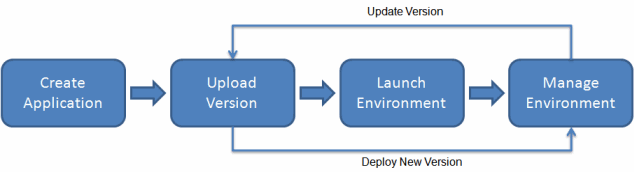
\includegraphics[width=0.5\textwidth]{figures/04_implementation/eb_flowchart}
    \caption[AWS Elastic Beanstalk Application Deployment]{AWS Elastic Beanstalk Application Deployment (source~\protect\cite{elasticbeanstalk})}
\end{figure}

It is important that the EB application runs in the same availability zone of the VPC as JIRA, otherwise it wouldn't be reachable at all.

The database runs on a managed Amazon RDS (Relational Database Service), which is a fast, secure and scalable deployment of a database engine. It manages backups, software patching, automatic failure detection, and recovery. The default database engine is MySQL.

\subsection{Spring Boot}

I first tried to use the play2 framework for educational purposes, but I encountered too many obstacles deploying the play2 application to AWS: 

\begin{itemize}
	\item It does not support WAR packaging.\footnote{There is an unofficial tool that packages the code in a WAR file, but it is not recommended for a production environment. Being constrained by a highly regulated market, something that already says that it is not production ready is an instant "No thanks".}
	\item It is not possible to run play2 packages (packaged by Activator tool) on a Tomcat Server.
	\item It comes with its own Netty Server, which is really clumsy to set up in an AWS environment.
\end{itemize}

All three combined resulted in an inability to synchronize the play2 application on port 9000 and NGINX running on port 5000. Unfortunately the Netty Server does not support compile-time port configuration and NGINX does not support running Activator to set up the port during run-time, so I had to drop the idea of using play2 as I was simply unable to deploy the application. After researching and discussing with my peers and coworkers, I looked up Spring MVC and stumbled upon Spring Boot, also recommended by my classmate. I tried a few sample apps and found out that it supports WAR packaging, runs natively on Tomcat and comes with almost the same perks as play2. I was ready to give it a try.

The primary goals of Spring Boot are:

"Spring Boot aims to make it easy to create Spring-powered, production-grade applications and services with minimum fuss. It takes an opinionated view of the Spring platform so that new and existing users can quickly get to the bits they need." \cite{spring-boot-blog}

\begin{itemize}
	\item Provide a radically faster and widely accessible getting started experience for all Spring development.
	\item Be opinionated out of the box, but get out of the way quickly as requirements start to diverge from the defaults.
	\item Provide a range of non-functional features that are common to large classes of projects (e.g. embedded servers, security, metrics, health checks, externalized configuration).
	\item Absolutely no code generation and no requirement for XML configuration.
\end{itemize}

\begin{figure}[!ht]
	\centering
	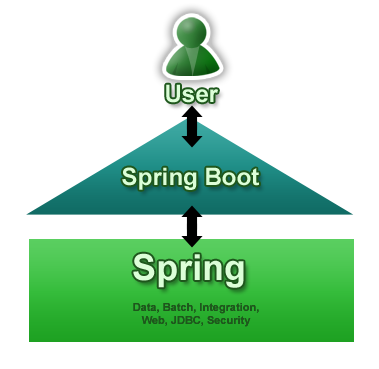
\includegraphics[width=0.4\textwidth]{figures/04_implementation/spring}
    \caption[Spring Boot architecture]{Spring Boot architecture (source~\protect\cite{spring-boot-doc})}
\end{figure}

The advantages seemed to be strong, the development environment was convenient (native support in IntelliJ IDEA) and after some validation from Amazon support regarding AWS EB deployment in our VPC environment, I was confident this would be a good choice.

\subsection{Workflow}

The server makes the workflow very easy and exposes a REST API to obtain the information. The basic workflow is as follows:

\begin{enumerate}
	\item List available projects.
	\item List available issues in a project, along with parsed watched values.
	\item Prepare a configuration XML file (streamed as a UTF8 encoded string) with selected issues.
\end{enumerate}

No registration or other setup is necessary - it runs in the VPC environment, so only the employees can access it with their approved devices with the network certificates. Also, JIRA is open for everybody to read, so why bother with extra signing in/out and session management, if it's actually not desired. The component works as-is and serves only one purpose: to connect JIRA and the application code as easily as possible.

\newpage

\subsection{Technologies Used}

In order to make the development as comfortable as possible, I used various open-source frameworks/technologies to help me out with things that would otherwise take a lot of time.

\subsubsection{H2 Database}

H2 is a Java SQL database that I used in in-memory mode during the development (before switching to RDS). It is great for fast prototyping and validating of design ideas before using the production database (RDS). Due to the fact that the entire database is deleted after a server is restarted, it enabled me to quickly change the schema without the need to do tedious database wipes. 

Another great thing is that it only needs to be defined in pom.xml and all other linking is provided out-of-the-box:

\bigbreak

\begin{lstlisting}
<dependency>
    <groupId>com.h2database</groupId>
    <artifactId>h2</artifactId>
</dependency>
\end{lstlisting}

Important note: as it wires up all connections automatically, it is absolutely vital not to have {\bf any other} database engine loaded via Maven, otherwise it crashes on start-up of Tomcat.

\subsubsection{Flyway}

Flyway is an open-source database migration tool. It aims to be clean and simple rather than robust and too complex. It uses six main commands:

\begin{enumerate}
	\item Migrate - Migrates the schema to the latest version.
	\item Clean - Drops all objects in the configured schemas.
	\item Info - Prints the details and status information about all the migrations.
	\item Validate - Validates the applied migrations against the available ones.
	\item Baseline - Baselines an existing database, excluding all migrations up to and including baselineVersion.
	\item Repair - Repairs the metadata table.
\end{enumerate}

Since I didn't need to migrate the database, thanks to the flexibility of H2, I mainly used Flyway for cold start (empty database). I defined what would be in the database after the server had started and Flyway filled it up for me.

\newpage

\subsection{Code Deployment}

The code is packaged by Maven and deployed as a WAR file to AWS EB instance, running a Tomcat 8 server. There is no need to configure anything with regards to basic networking - AWS EB is a back-to-back fully managed Platform as a Service (PaaS). Once deployed to VPC, the only thing that needs to be addressed is the availability zone - making sure it runs in the same zone as JIRA so they can communicate. It can be set up very quickly in the configuration section; however it can cause some frustration at the beginning when the developer doesn't know about it.

\bigbreak

There are multiple things to consider when deploying to AWS EB, even though it seems "super-easy" in most instructional videos and ads:

\begin{enumerate}
	\item Contrary to programmer's logic, one first has to create an "Application" and under that custom "Environments". In other words, Application is the main context, and environments are servers running in the same context, by default having the permission to communicate between each other.
	\item In Environment setup, we can choose either a Web Server Environment or a Worker Environment. Web Server is the hub of any application and is used in both Semantic Data Manager and Tracking Engine. Workers are only used in Tracking Engine and will be explained later.
	\item The chosen configuration was obviously Tomcat and I also opted for automatic load balancing and scaling.
	\item Opting to automatically create an RDS instance along with the environment is a really bad design. Once an environment is terminated, so is the database instance, which causes a serious data loss.
	\item In order to access the servers via SSH, it is necessary to define an EC2 Security Group and assign it accordingly. Otherwise, all outside access is prohibited.
	\item It is also crucial to choose the instance type wisely. I opted for m3.medium, because Java applications by themselves are quite demanding and I didn't want to risk being on the edge when strange errors occur because of insufficient memory capacity.
	\item Permissions and roles are absolutely crucial when you want to connect the Environment with other AWS services, such as object storage (S3 = Simple Storage Service) or a messaging queue (SQS = Simple Queue Service).
\end{enumerate}

 The size of the instance is recommended for any application running JVM. The configuration is Intel Xeon E5-2670 v2 (Ivy Bridge), 4GB SSD storage and 3.75GB RAM. Any additional memory is handled via S3.

\subsection{User Interface}

As mentioned before, Semantic Data Manager provides a REST API to be consumed by any kind of client capable of HTTP requests. Because my specialization is mobile applications, I chose to implement a mobile application for iOS as an administrating user interface for this component.

\subsubsection{Application Flow}

\begin{figure}[!ht]
	\centering
	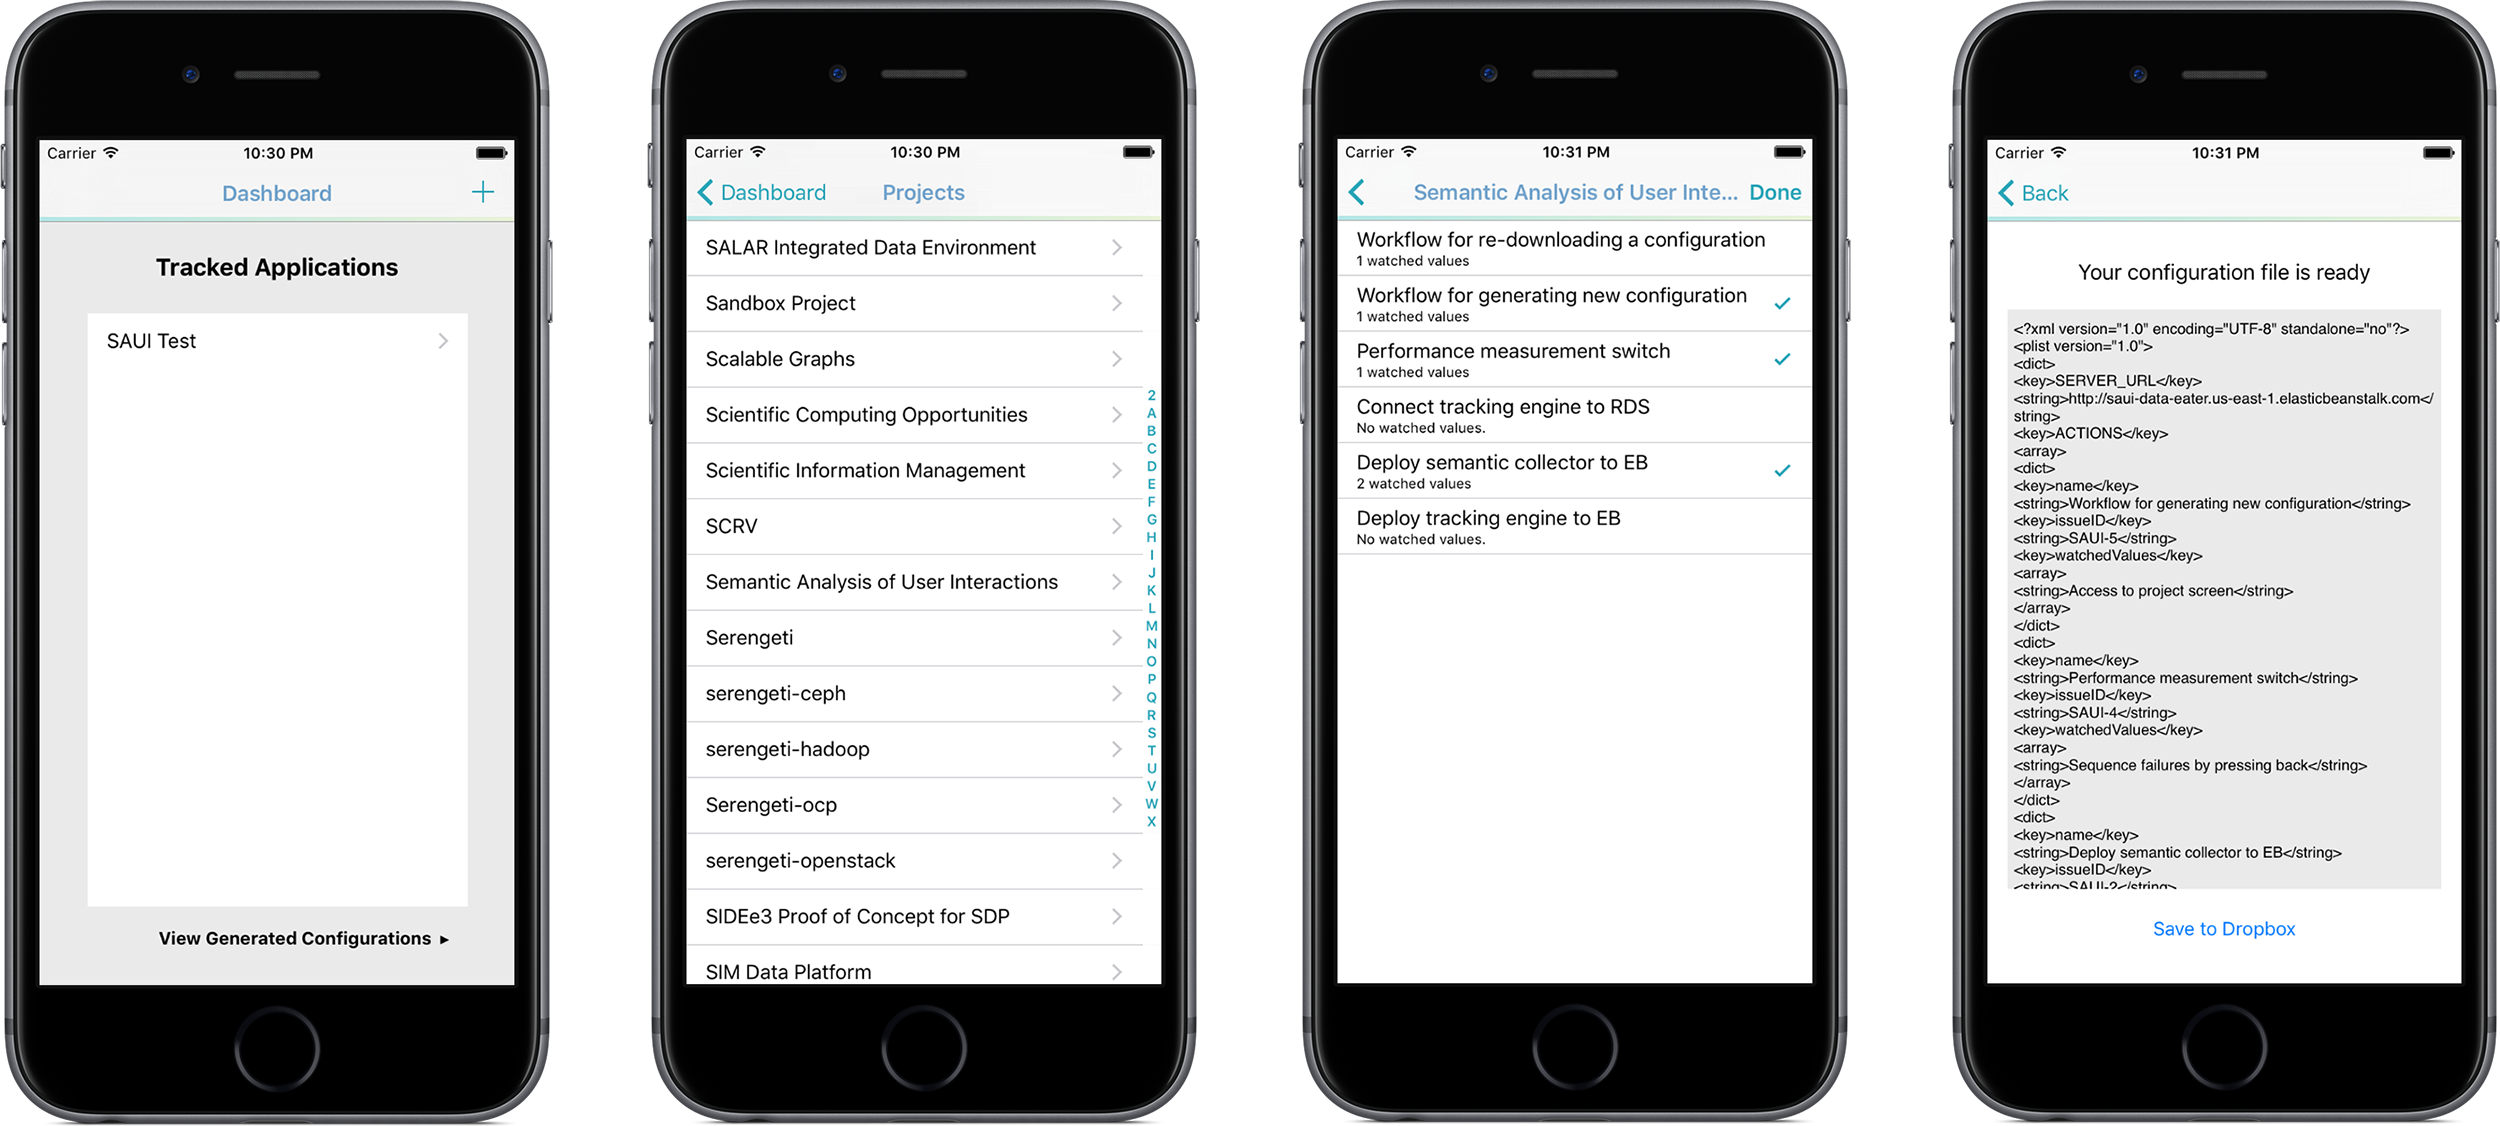
\includegraphics[width=0.95\textwidth]{figures/04_implementation/add_flow}
    \caption{Application Flow for Adding Configuration}
\end{figure}

\paragraph{Creating a new configuration}

\begin{itemize}
	\item The first screen presents the user with currently tracked applications and two actionable items - an add button and previously generated configurations. The add button leads to the next step in order to generate a new configuration.
	\item The second screen has all available projects in a list, scrollable with an alphabet index on the side. Naturally, selecting one leads to the next step.
	\item The third screen shows all available issues along with their watched values. The user is free to choose which one should be in the configuration (multiple-choice selection). When ready, the button "Done" proceeds with the process.
	\item The last screen shows the final configuration file that has been saved on the device. In order to send it to a computer, Dropbox integration has been implemented. When teams cooperate, it allows the user to automatically deliver the configuration file to all members of the team.
\end{itemize}

\newpage

\begin{figure}[!ht]
	\centering
	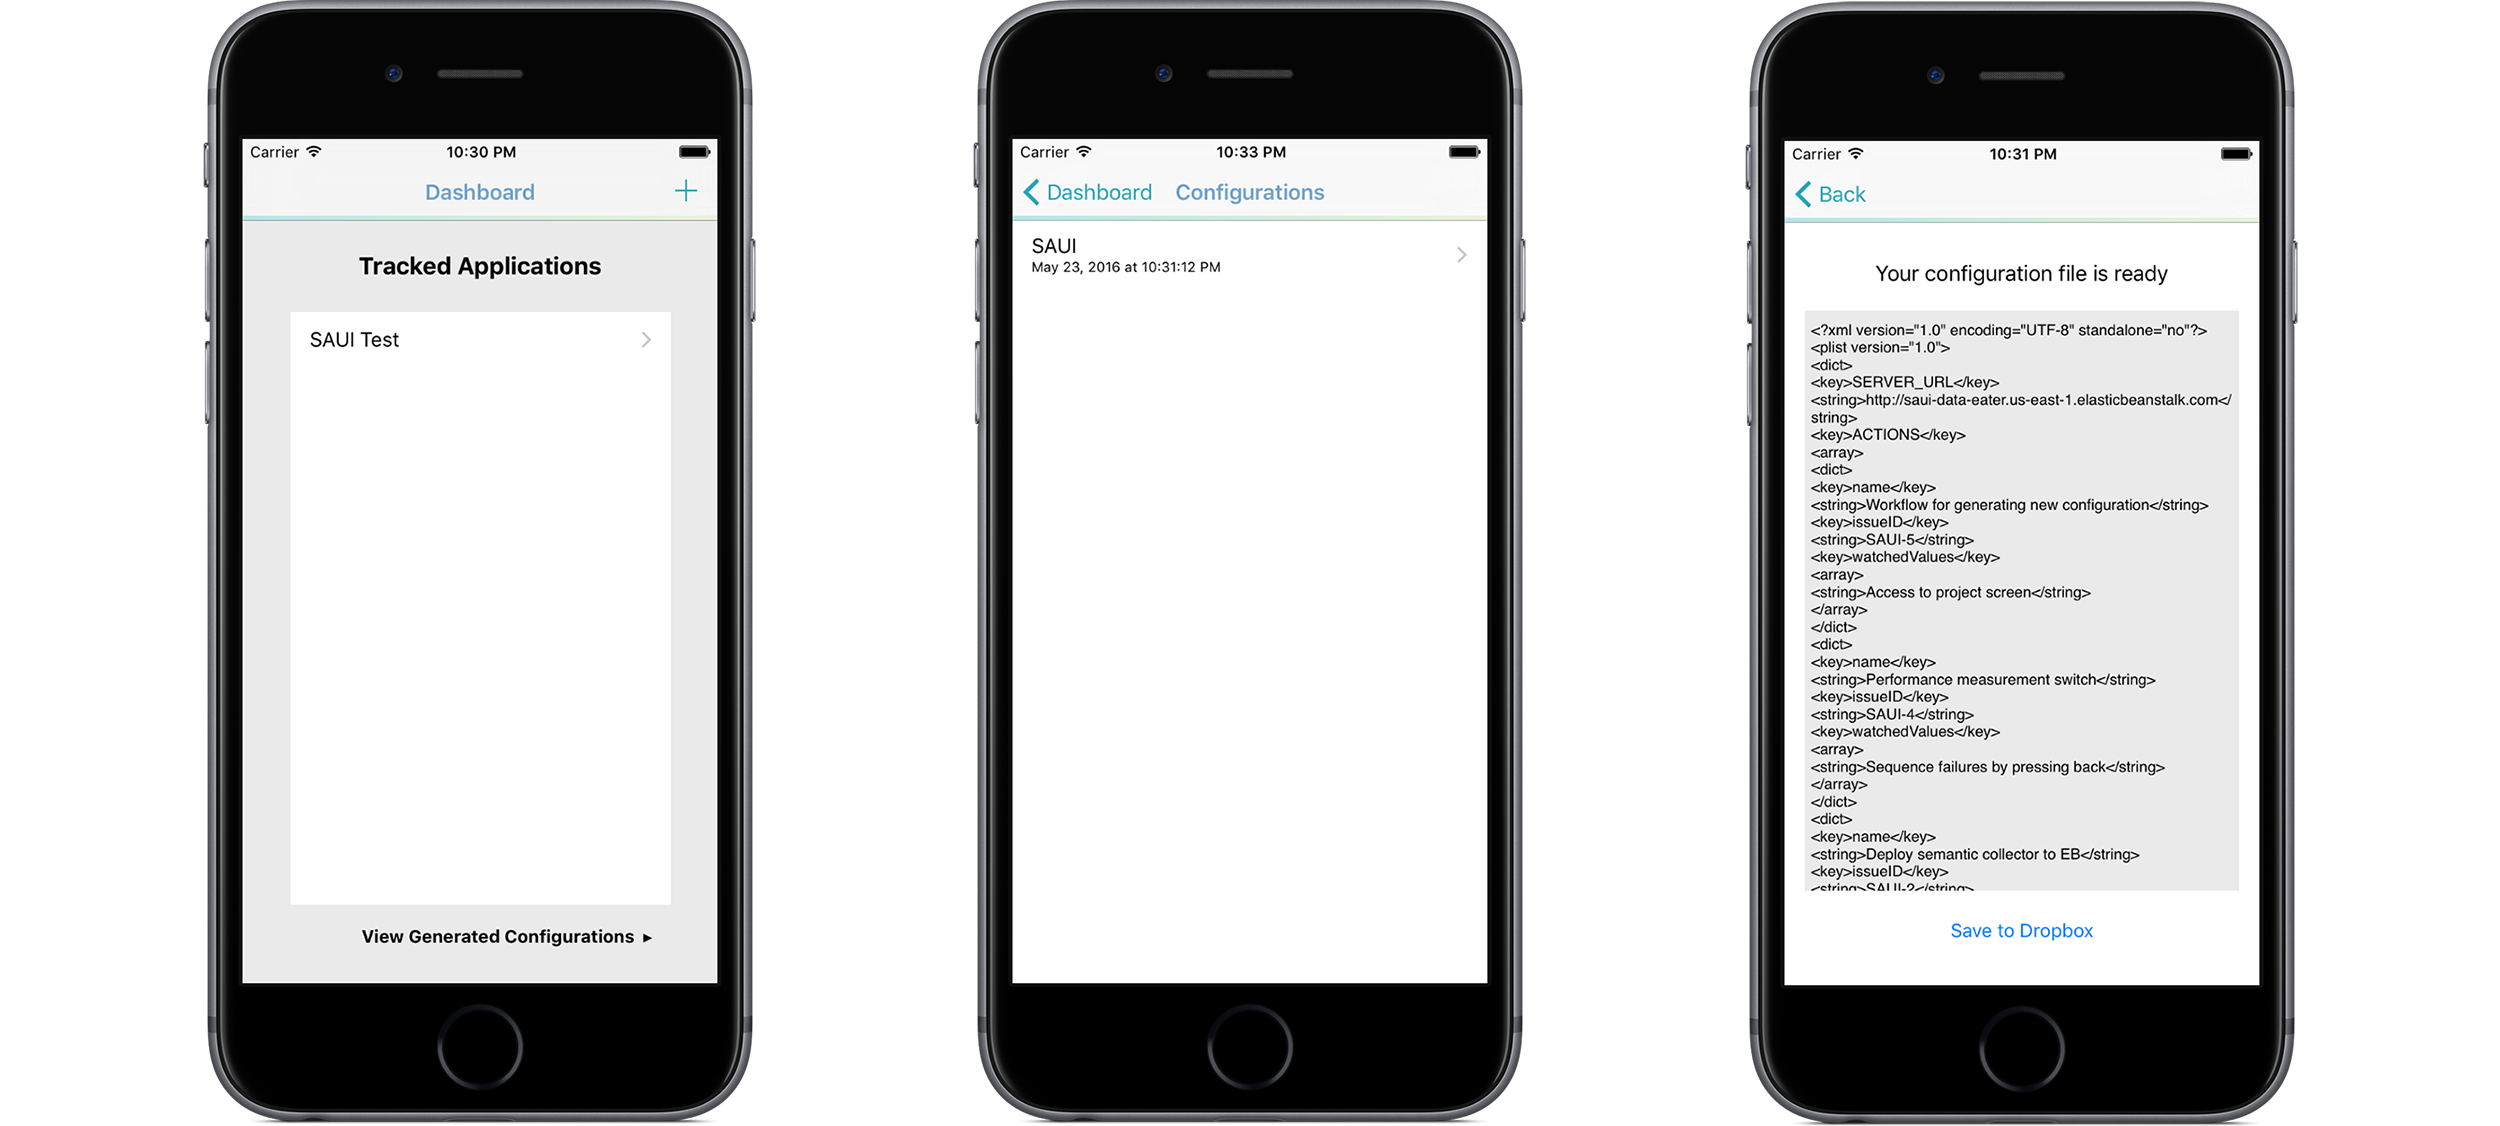
\includegraphics[width=0.95\textwidth]{figures/04_implementation/reconfig_flow}
    \caption{Application Flow for Recreating a Configuration}
\end{figure}

\paragraph{Recreating a previously generated configuration}

\begin{itemize}
	\item Instead of using the "Add" button, the user proceeds with the "View Generated Configurations".
	\item The second screen shows previously generated configurations. Those are immutable, because they are snapshots in time. They can only be re-downloaded again. If metadata has changed on JIRA, it is automatically updated.
	\item As the issue list is immutable in previously generated configurations, the user is automatically redirected to the last screen with the generated configuration file.
\end{itemize}

\begin{figure}[!ht]
	\centering
	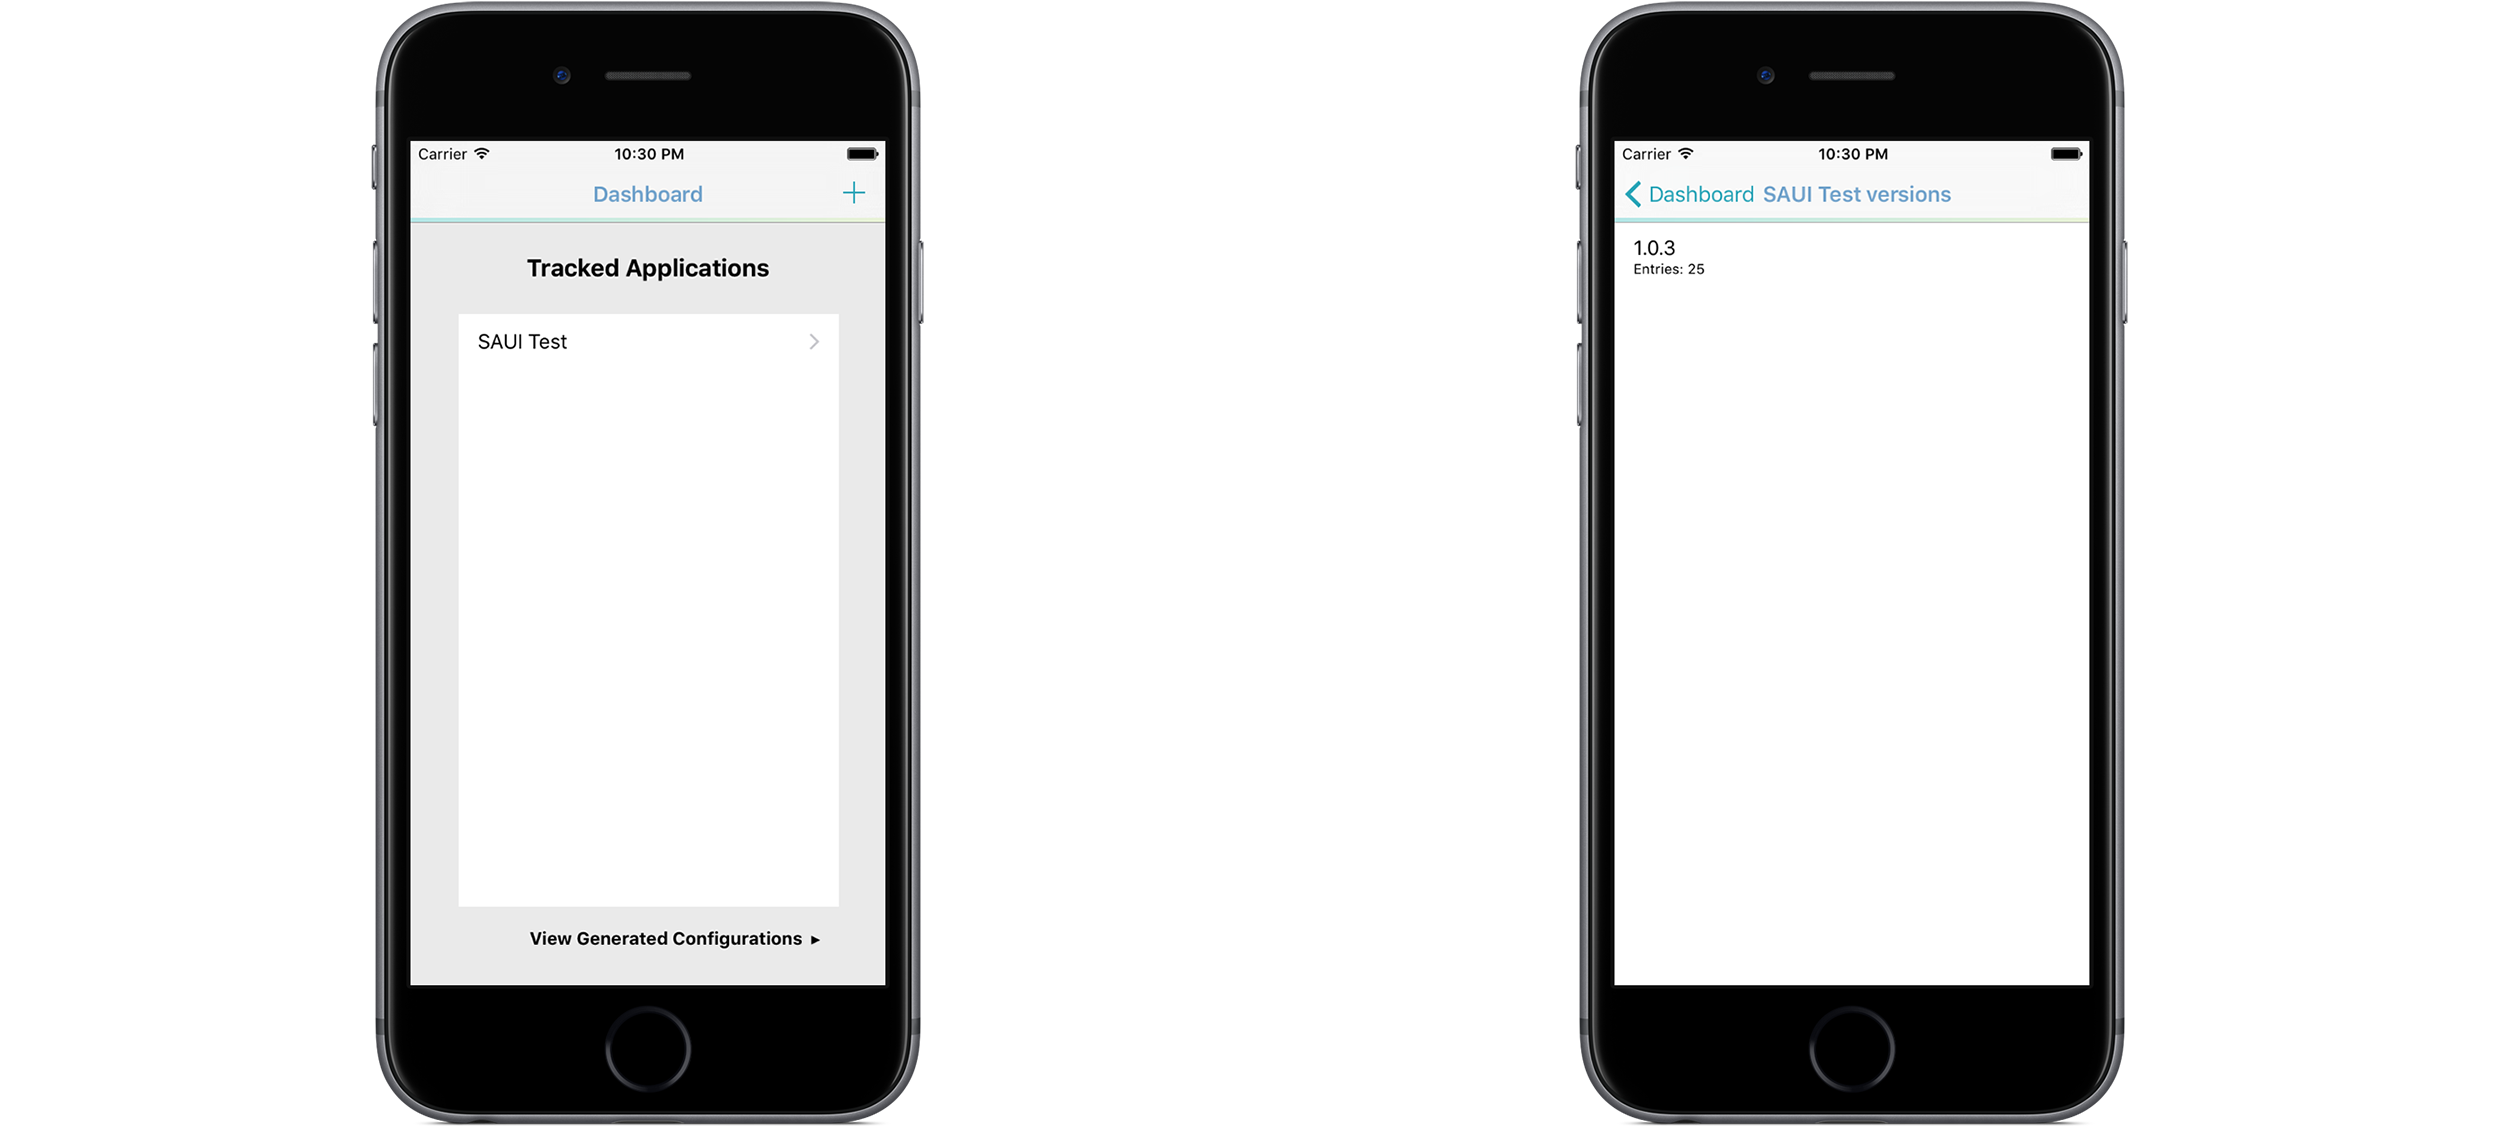
\includegraphics[width=0.95\textwidth]{figures/04_implementation/quick_summary}
    \caption{Application Flow for a Quick Overview of Gathered Data}
\end{figure}

\paragraph{Quick overview of gathered data}

\begin{itemize}
	\item Tapping on an application in the list of Tracked Applications leads to a quick overview of gathered data.
	\item The quick list of overview data is a simple list of the application's versions and the number of entries for each version. This application doesn't serve as a statistical front-end; this screen only serves as a quick overview for the user to know the current configuration status in the applications.
\end{itemize}

\subsubsection{Technologies Used}

\paragraph{Moya}\mbox{}\\
Moya\footnote{\url{https://github.com/Moya/Moya}} is an abstraction layer above an open-source networking library Alamofire\footnote{\url{https://github.com/Alamofire/Alamofire}}. It not only forces a cleaner code structure, but also makes it very easily testable as it is a single gateway to the internet.

The main advantages are:

\begin{enumerate}
	\item Compile-time checking for correct API endpoint accesses.
	\item Ability to define a clear usage of different endpoints with associated enum values.
\end{enumerate}

\paragraph{SwiftyDropbox}\mbox{}\\
SwiftyDropbox\footnote{\url{https://github.com/dropbox/SwiftyDropbox}} is an official framework for iOS to integrate Dropbox functionality directly into the application. In order to use it, it is necessary to register the application in the Dropbox Developer Console. Personal usage requires no review by the Dropbox team, though fully integrated usage does. For the purposes of this thesis, personal was sufficient.

\bigbreak

Both Moya and SwiftyDropbox are distributed via a standard dependency management tool Cocoapods, which is a similar dependency tool to Maven or Gradle for Java. Written in Ruby, it is less verbose and therefore the dependency management file is fairly short (MBProgressHUD\footnote{\url{https://github.com/jdg/MBProgressHUD}} is a "loading" dialog when a network operation is in process):

\bigbreak

\begin{lstlisting}
platform :ios, '9.0'
use_frameworks!

pod 'Moya'
pod 'SwiftyDropbox', '~> 3.0.0'
pod 'MBProgressHUD', '~> 0.9.1'
\end{lstlisting}

\newpage

\paragraph{Implementation Speciality}\mbox{}\\

Swift is a multi-paradigm language and allows the combination of an object-oriented programming approach and a functional programming approach. Because it was released in 2014 and doesn’t carry any legacy code along with it, it has these features all built in, along with proper generics and type safety rules. 

In one of the views (multiple-choice selection of issues), I had an interesting problem that I solved with a combination of the two paradigms mentioned. The situation was that I had a list of immutable Issue objects representing the data displayed in the list. In order to keep track of which cells had been selected, I had to create another separate array containing boolean values, representing selected/unselected. This is important, because the list view is dynamically generated and not keeping the record somewhere results in complete loss of selection on scroll, as the cells are generated as the user scrolls down/up. Unfortunately this results in having to perform manual filtering through the issues after the user is done selecting them. This is where the multi-paradigm comes in:

\bigbreak

\begin{lstlisting}
// declaration of properties - when issues are set after downloading, selectedIndicies is populated with false.

var selectedIndicies: [Bool] = []
var issues: [Dictionary<String, AnyObject>] = [] {
    didSet {
        selectedIndicies = [Bool](count:issues.count, repeatedValue: false)
    }
}

// filtering

let result = zip(self.issues, self.selectedIndicies).filter{$0.1}.map{$0.0}

// which the same as its longer version

let result2 = zip(self.issues, self.selectedIndicies)
	.filter{ (sequence: (object: Dictionary<String, AnyObject>, isSelected: Bool)) -> Bool in
		return object.isSelected
	}.map{ (filteredSequence: (object: String, isSelected: Bool)) -> String in
		return filteredSequence.object
	}


\end{lstlisting}

\bigbreak

This feature of the language is great, because it keeps the code clear and structured. There is absolutely no need for long and verbose code structures, using for-cycles and being afraid that it might exceed the maximum index of an array. Also, the global functions on collections are better optimized by the compiler, resulting in 100\% speed increase of collection operations.\footnote{\url{http://stackoverflow.com/questions/29301577/performance-issue-while-finding-min-and-max-with-functional-approach/29305300\#29305300}}

\newpage

\section{Tracking Engine}

\begin{figure}[!ht]
	\centering
	\includegraphics[width=0.8\textwidth]{figures/04_implementation/tracking_diagram}
    \caption{Tracking Engine Diagram}
\end{figure}

Tracking Engine is also deployed in AWS EB but its workflow is a bit more complex. The whole system is designed to be horizontally scalable on every component:

\begin{enumerate}
	\item {\bf Gateway} is scaled automatically by the Elastic Beanstalk environment.
	\item {\bf S3 and SQS} are scaled automatically by AWS.
	\item {\bf Aurora DB} is scaled automatically by AWS, along with replication and availability.
	\item {\bf Workers} are scaled automatically instance to instance (vertical scaling), or can be deployed multiple times as necessary (horizontal scaling - in the console, simply choose "Clone Environment"). Sometimes it is cheaper to deploy more workers on less powerful instances instead of letting it scale automatically with just a few.
\end{enumerate}

\subsection{Workflow}

The gateway is written in Java, also using the Spring-Boot framework. It's the main intersection for all the requests coming in and out. The workers are also another Spring-Boot application (deployed multiple times). Both of the applications use AWS SDK for connecting to S3 and the Aurora Database. The queue is implemented automatically in Amazon's environment and the only thing that a developer has to define is the method called on the worker (using HTTP POST). If the worker returns "200 OK", the message is considered to have been processed, so it is crucial to really throw an exception if one occurs, otherwise the message is lost.

\newpage

The general workflow is as follows:

\begin{enumerate}
	\item When a client application sends in the stats of usage, the procedure is designed to save as much data as possible - data is sent archived using GZIP\footnote{\url{http://www.gzip.org/}}. Because the data is serialized into a JSON file, GZIP performs really well and saves over 90\% of data otherwise spent on sending the giant list of events.
	\item The gateway server takes the archive as it is and saves it to S3 object storage.
	\item After uploading the archive, the gateway server sends a message into the task queue SQS. The message is absolutely straight-forward, containing only the name of the file. The name of the file is generated by the gateway server using the UUID library. If that's not enough, S3 makes sure there is never a collision in the names - if there is, it proposes a different name and returns it after the upload, so it's always unique.
	\item SQS then tries to deliver the message to an available worker. If it cannot be delivered it ends up "in flight", which is Amazon's implementation of a dead letter queue. From there the task queue system tries to deliver with a lowering frequency.
	\item When the message is delivered to the worker, it obtains the archive from S3, unzips it, parses and saves to the database. When done, it also removes the archive from S3. Then it confirms with "200 OK", marking that the message has been successfully processed.
\end{enumerate}

\subsection{Aurora Database}

Amazon Aurora is a fully managed, MySQL-compatible, relational database engine that combines the speed and reliability of high-end commercial databases with the simplicity and cost-effectiveness of open-source databases. It delivers up to five times the performance of MySQL.

\begin{figure}[!ht]
	\centering
	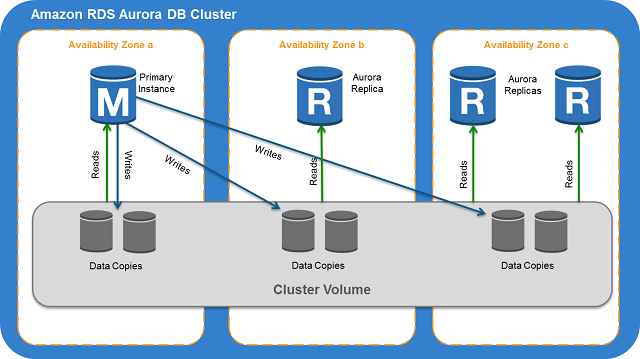
\includegraphics[width=0.6\textwidth]{figures/04_implementation/aurora}
    \caption[Aurora Replication Flow]{Aurora Replication Flow (source~\protect\cite{aurora})}
\end{figure}

\newpage

Every application operating with large volumes of data eventually comes up against a bottleneck in the database. I decided not to compromise when I was choosing between database engines. There was also a simple RDS instance available, just like the one I am using in the Semantic Data Manager, but this one will have exponentially more entries in the database then the Semantic Data Manager ever will.

Interestingly enough, Aurora DB wasn't officially supported by the jdbc library enabling applications to connect to it. I managed to find it was in the Release Candidate 2 of version 1.1.0 of the library. 

\bigbreak

\begin{lstlisting}
<dependency>
	<groupId>org.springframework.cloud</groupId>
	<artifactId>spring-cloud-aws-jdbc</artifactId>
	<version>1.1.0.RC2</version>
</dependency>
\end{lstlisting}

\bigbreak

The release of the official update is scheduled for June 2016.

\subsection{Deployment}

The networking capabilities of AWS are very broad and because the architecture of the Tracking Engine is quite complex, it is important to first introduce a couple entities in the AWS cloud environment.

\subsubsection*{Identity and Access Management}

Identity and Access Management (= IAM) is a web service that allows the management of access to compute, storage, database and application services in the AWS cloud. It uses concepts known in other similar services in different environments - Users, Groups and Permissions. It is very detailed and allows specification of which users have access to certain services, the kinds of actions they can perform and which resources are available (ranging from virtual machines, database instances and even the ability to filter database query results). The good thing is that it works seamlessly with existing identity management solutions, such as Active Directory\footnote{\url{https://technet.microsoft.com/en-us/library/dd448614.aspx}}

\subsubsection*{Permissions}

Permissions allow specification of who has access to AWS resources and what actions can be performed on those resources. Every IAM user starts with no permissions at all. In other words, by default, users can do nothing, not even view their own access keys. Permissions can be added to the user (attach a policy to the user) or the user can be assigned to a group that has the desired permissions.

\newpage

Permissions can be assigned either as identity-based or as resource-based:

\begin{itemize}
	\item Identity-based, or IAM permissions are attached to an IAM user, group, or role and allow specification of what that user, group, or role can do.
	\item Resource-based permissions are attached to a resource. Resource-based permissions allow specification of who has access to the resource (S3, SQS) and what actions they can perform on it. Resource-based policies are inline only, not managed.
\end{itemize}

\subsubsection*{Policies}

To assign permissions to a user, group, role or resource, a policy has to be created. A policy is a document that explicitly lists permissions.

A policy allows specification of the following:

\begin{itemize}
	\item Actions: which actions should be allowed. Every service has its own set of actions.
	\item Resources: which resources it should be allowed to perform actions on.
	\item Effect: which effect will a request to access by a user generate - deny or allow.
\end{itemize}

All policies are defined by a JSON file and can be assigned in a totally granular fashion to every service and user.


\subsubsection*{Security Group}

A security group acts as a virtual firewall that controls the traffic for one or more instances. When an instance is launched, it can be associated with one or more security groups. Each group has rules that can be added that allow traffic to or from its associated instances. All rules for a security group can be modified at any time. The new rules are automatically applied to all instances that are associated with the security group. When a decision has to be made whether to allow traffic to reach an instance, all the rules from all the security groups associated with the instance are evaluated.

\bigbreak

The whole AWS cloud environment is very complex and has much more to offer than just the couple points I listed above. For the sake of deploying my architecture it is sufficient. For anything else, AWS documentation\footnote{\url{http://docs.aws.amazon.com/IAM/latest/UserGuide/introduction.html}} is of very high quality and virtually any question can be found there.

\newpage

Now that I have established all the necessary foundations of the inner workflow in AWS, all of these prerequisites have to be met in order to deploy the Tracking Engine:

\begin{enumerate}
	\item AWS EB application with IAM role with permissions to access SQS and S3.
	\item Policy on S3 for the IAM role set up to be able to read/write via JSON configuration:
	
\begin{lstlisting}
"Statement": [
		{
			"Sid": "sid123456789",
			"Effect": "Allow",
			"Principal": "*",
			"Action": "s3:*",
			"Resource": [
				"arn:aws:s3:::iam-role-name/*",
				"arn:aws:s3:::iam-role-name"
			]
		}
	]
\end{lstlisting}	
	
	\item Aurora Database instance up and running with the same Security Group as the AWS EB application.
	\item Open 3306 port in the Security Group between the AWS EB application and the Aurora Database.
\end{enumerate}

Everything else is automatic when the AWS EB application is set up as described with the Semantic Data Manager. The database URL is for security reasons injected through environment variables (it should never be hard-coded!).

\subsection{Timeseries Application}

The administration application for the Semantic Data Manager does provide a quick overview, but that is not meant to serve as a dashboard or any decision-making helper tool. It's merely indicates whether or not the desired application version is being tracked. Clearly that is not optimal for deriving any conclusions.

In order to show the power of the data gathered, I developed another mobile application meant just for displaying the flow of the data in time. It is inspired by the popular application Numerous\footnote{\url{http://numerousapp.com/}}, available on the Apple App Store.

The requirements for such an application could be endless - graph mash-ups, benchmarking and so much more. In order to simply demonstrate the movement in the KPIs and the potential in the data, I chose to display the total increase/decrease of entries during the last five days.

\newpage

\begin{figure}[!ht]
	\centering
	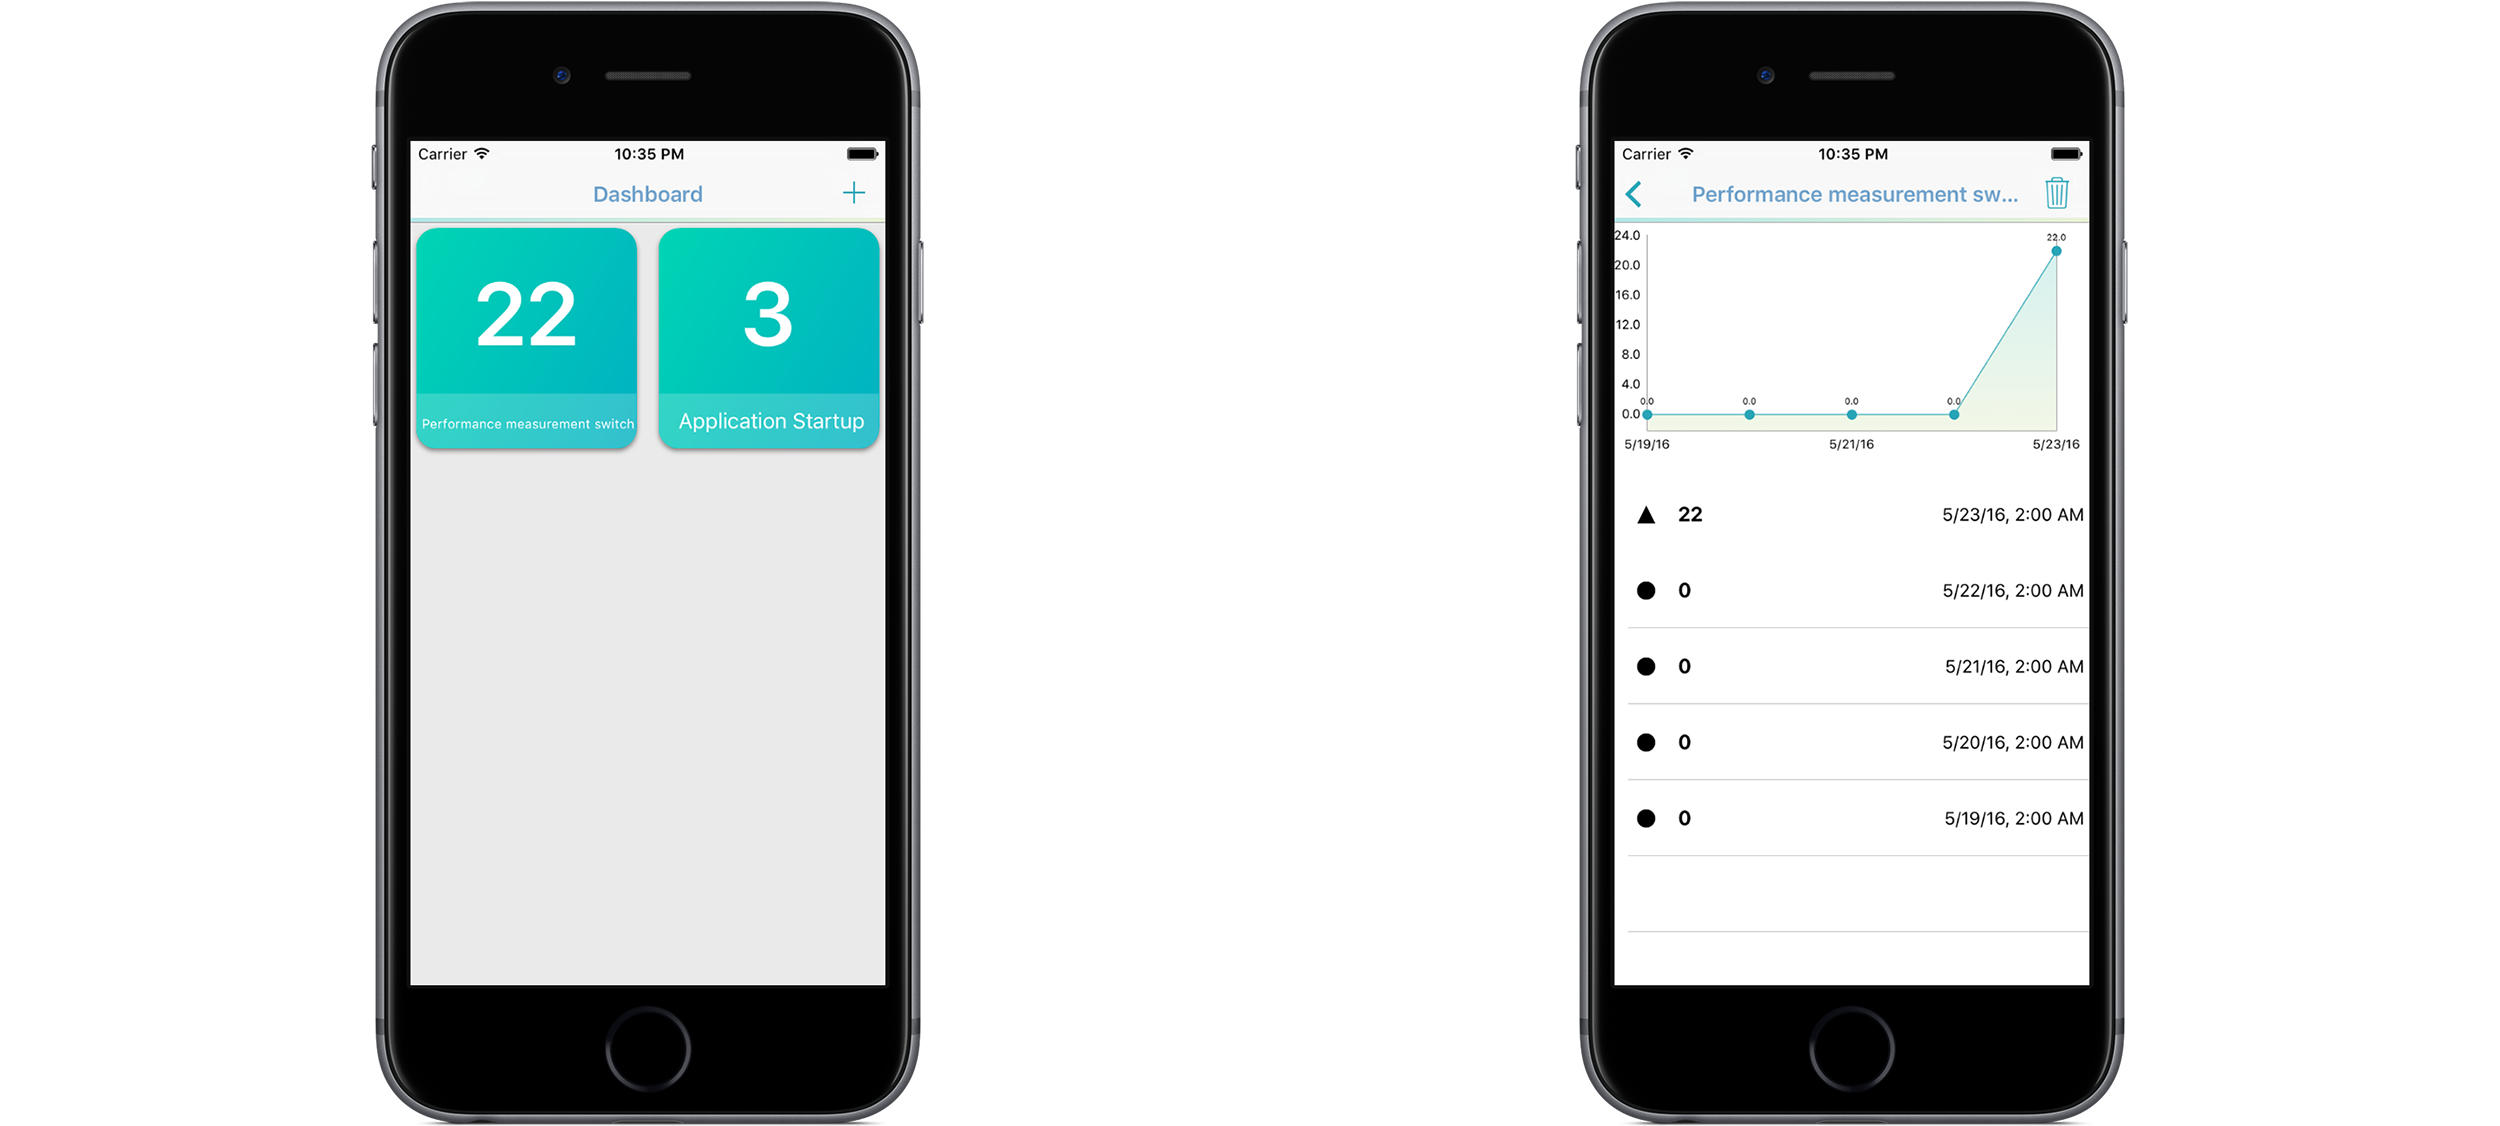
\includegraphics[width=0.95\textwidth]{figures/04_implementation/time_flow}
    \caption{Time Series Detail}
\end{figure}

\begin{enumerate}
	\item Once an application has been chosen using the "Add" button (the list looks identical to any previous lists), the application automatically loads all KPIs available on the server. The number marks the total number of entries in the last five days.
	\item Tapping on a number in the grid displays a detailed graph showing the total number of entries per day - adding up to the same number as is displayed on the dashboard. The KPI can be deleted from the application so it's not displayed anymore (it remains on the server), because the application persists what was selected in the choice of applications and refreshes it on the next start of the application.
\end{enumerate}

\subsubsection{Technologies Used}

Aside from the technologies already listed in the administration application (which I have used again), namely Moya and MBProgressHUD, I also used:

\paragraph{ios-charts}\mbox{}\\

ios-charts is a charting library based on MPAndroidChart\footnote{\url{https://github.com/danielgindi/Charts}}. It is written in Swift and supports a plethora of chart types - line charts, bar charts, pie charts, scatter plots, box plots, bubble charts and radar charts.

The setup is quite "procedural" and requires a lot of boilerplate code, but when it's well set up, the result is very satisfying.

\newpage

\paragraph{Realm.io Database}\mbox{}\\

Realm is a mobile database made by a start-up of the same name. Developed by two engineers from Nokia - Alexander Stigsen and Bjarne Christiansen, it is currently one of the most widely used frameworks for iOS development. 

The main advantages are:

\begin{itemize}
	\item Mobile-first: built from the ground up to run directly inside phones, tablets and wearables.
	\item Simple: data is directly exposed as objects and queryable by code.
	\item Fast: Realm is faster than SQLite for common operations.
\end{itemize}

The great thing in comparison to CoreData, a native Apple framework on top of SQLite, is not having to keep the context object everywhere, where something should be written in the database. Another great tool shipped with the framework is a migration tool that has a similar philosophy to Flyway, which I described above.

\subsubsection{API Used}

Obviously, the goal is to send the data in as condensed a format as possible. For those reasons, the automatically exposed API by Spring-Boot was too verbose. In order to load the data, I created another Controller endpoint in the Tracking Engine application that handles special requests from the Timeseries application:

\begin{enumerate}
	\item \emph{/mobile/applicationEntryTypes} - returns a list of all KPIs in an application.
	
\begin{lstlisting}
{ "entryTypes" : [
		{"applicationName":"SAUI Test","applicationVersion":"1.0.3","name":"Performance measurement switch","total":12654}
	]
}	
\end{lstlisting}	
	
	\item \emph{/mobile/applicationEntrySummary} - returns five-day entry count for a given KPI.
	
\begin{lstlisting}
{ "entries":[ ... ],
  "metadata":[
		{"entries":11,"timestamp":1464048000}, ...
	]
}
\end{lstlisting}	
\end{enumerate}

\newpage

\section{Tracked Device SDK}

In order to integrate the domain vocabulary generated by the Semantic Data Manager, it is necessary to have an interpreter of such vocabulary. For the implementation for Apple devices, I chose native development in Swift.

As stated in the previous chapter, the SDK has two layers - the configuration interpreter and an interface to log an event.

\subsection{Interpreter}

The interpreter enables the storing interface to call functions on it that extract the information from the configuration file, without the need to handle the low-level file access. It is made to be as precise as possible - no errors allowed. When the configuration file is not present it calls a system level fatalError function. 

Methods exposed:

\begin{itemize}
	\item \emph{getDictionary} - returns the whole configuration file as a dictionary object
	\item \emph{getURL} - returns the URL of the Tracking Engine
	\item \emph{getAllActions} - returns all actions available in the dictionary
\end{itemize}

\subsection{Interface for Storing}

The interface for storing provides a couple functions:

\begin{enumerate}
	\item \emph{startEvent(itemIndex: Int)} - logs the beginning of an event on the given index in the configuration.
	\item \emph{finishEvent(itemIndex: Int)} - logs the end of an event on the given index in the configuration.
	\item \emph{watchValue(itemIndex: Int, valueIndex: Int)} - logs an action of watched value on the given index assigned to an event on the given index in the configuration.
	\item \emph{reportData(compressed: Bool, success: (() -> Void)?)} - reports data to the server, either in compressed format or not and after finishing, it calls the optional (not mandatory to use) completion closure.
\end{enumerate}

If an event is to be logged and the interpreter doesn't find it, fatalError is called again.

\newpage

To ensure clean code and the level of "security"\footnote{Security here refers to the Defensive Programming coding style leading to a reduced number of bugs and problems.} of the code, Swift's if-let and guard statements came in very handy:

\bigbreak

\begin{lstlisting}
func startEvent(itemIndex: Int) {
	guard let action = ConfigurationReader.getAllActions()[safe: itemIndex]
		else {
			fatalError("Action at given index (\(itemIndex)) does not exist!")
	}
        
	if let name = action["name"] as? String, issueID = action["issueID"] as? String {
		self.addEvent("START", name: name, issueID: issueID)
	} else {
		fatalError("Action at given index (\(itemIndex)) has details in wrong format!")
	}
}
\end{lstlisting}	

\bigbreak

The guard statement and the if-let statement are somewhat similar - they make sure that an object the developer is trying to access is not null and will not cause any problems. The main difference is that if-let goes inside curly brackets and creates more complexity by indented code. Guard statement allows in-line handling; however, it does not allow chaining of the statements like the if-let statement does.

In fact, an even more interesting feature is used in the code snippet above - Swift extension. The safe look-up of an action in the array of all actions is a separate function written as an extension to the standard collection functions in Swift. The extension is written this way:

\bigbreak

\begin{lstlisting}
extension Array {
    subscript (safe index: Int) -> Element? {
        return indices ~= index ? self[index] : nil
    }
}
\end{lstlisting}	

\bigbreak

There is no need to override the whole Array object and implement a new method. The compiler takes it as a new first-class function on the collection and it can be used in the whole project.

\newpage

\subsection{Distribution}

When a developer wants to use an external library, there are two standard ways how to incorporate it into the project:

\begin{enumerate}
	\item Cocoapods
	\item Carthage
\end{enumerate}

Cocoapods is more invasive - it links the source code into the project as another sub-target and creates a new workspace for Xcode. Sometimes it can be frustrating, especially during clean builds when having more than five dependencies can take five minutes or more to fully compile.

Carthage is a non-invasive way of importing dependencies; however, it is not standardized by Apple - it requires initial setup in Xcode and is liable to break during Xcode updates.

\bigbreak

The company standards required me to create both, that is, a Podspec file for Cocoapods and a Cart file for Carthage:

\begin{lstlisting}
// Cartfile
github "Moya/Moya" ~> 6.4.0
github "realm/realm-cocoa" ~> 0.99
github "nicklockwood/GZIP" ~> 1.1

//Podspec
Pod::Spec.new do |s|
  s.name         = "SAUI"
  s.version      = "1.0"
  s.summary      = "SAUI Swift framework for logging events."
  s.author             = { "Michal Svacha" => "svachmic@fel.cvut.cz" }
  s.ios.deployment_target = '8.0'
  s.osx.deployment_target = '10.9'
  s.watchos.deployment_target = '2.0'
  s.tvos.deployment_target = '9.0'
  s.source       = { :git => "https://url/SAUI-Swift.git", :tag => s.version }
  s.default_subspec = "Core"

  s.subspec "Core" do |ss|
    ss.source_files  = "Source/*.swift", "Source/Plugins/*swift"
    ss.dependency "Moya", "~> 6.4.0"
    ss.dependency "RealmSwift", "~> 0.99"
    ss.dependency "GZIP", "~> 1.1"
    ss.framework  = "Foundation"
  end
end

\end{lstlisting}	

\newpage

\subsection{Workflow}

The usage of the framework after linking is very straight forward. The main object to use is called \emph{Reporter} - it is singleton and accessible via it's property \emph{sharedInstance}. The Reporter class is the interface for storing and offers all methods listed in the previous section.

It can be initially set up whether the reporting to the server will be handled automatically or not. If not, the developer has to handle the upload scheduling himself and call the function \emph{reportData} whenever needed. If automatic reporting is set up, an NSTimer thread object runs in the background, firing every 120 seconds to check if there is anything in the database to be reported. If yes, it gets uploaded to the server.

\subsection{Technologies Used}

Aside from all the technologies previously listed (Moya and Realm), in this component I also had to use Alamofire (from which I tried to abstract myself away with Moya). Unfortunately Moya does not support uploading binary data via POST, so I had to use a lower-level tool to get the archived data to the server.

Another technology I used here is a GZIP \cite{deutsch1996gzip} library handling the archiving of data. The library comes with a choice of level of encryption, which for a text can be naturally selected to the highest number. The object that is archived can only be an NSData object, so I serialized the JSON that is supposed to be archived into UTF8-encoded data:

\bigbreak

\begin{lstlisting}
let jsonData = try! NSJSONSerialization.dataWithJSONObject(events, options: NSJSONWritingOptions.PrettyPrinted)
let archived = jsonData.gzippedDataWithCompressionLevel(1.0)!
\end{lstlisting}	


\chapter{Testing}

The whole system has many components and it is a widely accepted fact that the more complex the system is, the more prone to errors and bugs it is. In this chapter I will describe the benchmarking tests I performed on the most complex part - the tracking engine - and the user tests I performed not only on the front-end applications but also on the whole workflow of the system as well.

\section{Benchmark Tests}

To verify that the Tracking Engine handles an extensive load it is important to simulate a real-world peak that could occur during everyday usage. I identified the biggest bottlenecks to be the client side (networking issues like poor EDGE connection) and the workers' parsing job (how big a task can they manage?). The Gateway server has an automatic load-balancer, so there shouldn't be a problem, just like with all other automatically scaled components by Amazon (S3 and SQS).

\subsection{Workers}

To verify how big a load a single worker can handle, I created data on the front-end of various sizes and sent it to the server. I turned on a logging system, CloudWatch, that told me the precise times when a job started on a worker and when it finished.

\begin{table}[!ht]
\begin{center}
\begin{tabular}{|c|c|c|c|}
\hline
\textbf{Number of entries} & \textbf{Execution Start} & \textbf{Execution End} & \textbf{Duration} \\
\hline
100 & 15:46:35.966 & 15:46:41.595 & $5.629s$ \\
\hline
500 & 16:06:57.851 & 16:07:15.265 & $17.414s$ \\
\hline
1000 & 15:51:23.311 & 15:51:59.060 & $35.749s$ \\
\hline
5000 & N/A & N/A & N/A \\
\hline
10000 & N/A & N/A & N/A \\
\hline
\end{tabular}
\end{center}
\caption{Worker Processing Times}
\label{tab:table_worker}
\end{table}

\newpage

To give it a visual perspective:

\begin{figure}[!ht]
\begin{center}
\begin{tikzpicture}
    \begin{axis}[
    		height=7cm,
		width=0.85\textwidth,
		xlabel={Number of entries},
    		ylabel={Time to process (s)}
    	]
    \addplot coordinates { 
    		(100, 5.629) 
    		(500, 17.414) 
    		(1000, 35.749)};
    \end{axis}
\end{tikzpicture}
\end{center}
\caption{Worker Processing Times Graph}
\end{figure}

The graph itself doesn't show anything that would be out of the ordinary, so why did the workers fail to process 5000 and 10000 entries? The scenario of what actually happened is interesting in both cases and it isn't the fault of the workers themselves:

\begin{enumerate}
	\item {\bf 5000 entries: } When the first worker got the message to handle 5000 entries sitting on S3, he reached out for them and started parsing. However he did not make it in the given time of message execution and therefore the message was marked as failed. When the SQS tried to deliver it again, the worker was still processing the data and so it was sent to another worker, who started parsing them. Then finally the first worker returned "200 OK" which resulted in an inconsistent state and the whole system went into "Warning". CloudWatch stopped the servers and I couldn't get the execution times. The result was that, unfortunately, the data in the database was saved twice.
	\item {\bf 10000 entries: } In the last round, it simply took too long and the whole worker crashed and so did the second one soon after the first one.
\end{enumerate}

\subsubsection*{Conclusion}

Even though compression does save some data on the client side, it also introduces a new complexity on the server side that is very hard to parallelize, so it is important to find a "good enough" amount of entries to be uploaded in a single batch report.

\newpage

\subsection{Client-side Compression Rate}

To continue the search for optimum load on both sides, I measured the performance of the GZIP compression library. I performed it on a real device (iPhone 6S), using logging capabilities in Xcode. 

\begin{table}[!ht]
\begin{center}
\begin{tabular}{|c|c|c|c|}
\hline
\textbf{Number of entries} & \textbf{Before compression} & \textbf{After compression} & \textbf{Compression rate} \\
\hline
100 & 51.41kB & 0.67kB & 76.7x \\
\hline
500 & 252.98kB & 1.65kB & 153.3x \\
\hline
1000 & 504.92kB & 2.87kB & 177.8x \\
\hline
5000 & 2520.55kB & 12.65kB & 199.3x \\
\hline
10000 & 5040.08kB & 24.89kB & 202.5x \\
\hline
\end{tabular}
\end{center}
\caption{Client-side Compression Rate}
\label{tab:compression}
\end{table}

To give it a visual perspective:

\begin{figure}[!ht]
\begin{center}
\begin{tikzpicture}
    \begin{axis}[
    		height=7cm,
		width=0.85\textwidth,
		xlabel={Number of entries},
    		ylabel={Compression rate}
    	]
    \addplot coordinates { 
    		(100, 76.7) 
    		(500, 153.3) 
    		(1000, 177.8) 
    		(5000, 199.3) 
    		(10000, 202.5)};
    \end{axis}
\end{tikzpicture}
\end{center}
\caption{Compression Rate Graph}
\end{figure}

I was quite surprised by the performance, even though I expected it to be performing very well, given the fact that the JSON file structure is very repetitive. What I was equally suprised by was the logarithmic shape of the curve. In other words, I did not expect the compression rate to slow down.

\subsubsection*{Conclusion}

The best amount seems to be somewhere in the range 400 - 700 entries. Combined with the knowledge from the previous measurement (worker processing time) I would aim to be in lower numbers, perhaps 400 - 600. That ensures a very good compression rate (\textasciitilde 150x) and also good processing time on the backend (\textasciitilde 18s)

\newpage

\section{User Tests}

I performed user tests in three different ways:

\begin{enumerate}
	\item Personal interviews
	\item Scenario test
	\item Panel discussion
\end{enumerate}

Each tested different aspects of the whole solution and each brought me some new insights into which problems I had overlooked during the development.

\subsection{Personal Interviews}

The personal interviews were held with three different people, each from a different department. I showed them the whole workflow and asked them to give me feedback on anything they wanted.

\subsubsection{Test Setup}

The interviews were held in a company kitchen - an area where people relax, chat and hang out during their personal breaks. The work was presented on a laptop (JIRA workflow and the deployment in the AWS console, should it be of any interest) and an iPhone 6S. Both devices were directly accessible to the person being interviewed.

I extracted the highlights from each interview:

\begin{enumerate}
		\item Associate Director, Applied Technology
		\begin{itemize}
				\item[] "I like the fact that I define the domain vocabulary once. Once and that's it. That's great."
				\item[] "Could we wire-up the installation IDs to the user IDs to ensure that 10 installations on the same device are counted as one?"
				\item[] (Looking at the Timeseries Application) "Yes! That's exactly what I want to see."
		\end{itemize}			
		
		\item Mobile Application Development Lead
		\begin{itemize}
				\item[] "I didn't quite understand the concept of WATCH when you first said it, maybe name it differently, like "Event" for example?"
				\item[] "Is it possible to produce a user flow? Like how the user moves throughout the application?"
				\item[] "How do you address a change in the configuration file? Is there a way to ensure I am not reporting something I was reporting before?"
				\item[] "How do you ensure that the content is sent later if it fails? Are you using operations.io or some other framework?"
		\end{itemize}
		
		\item UX Lead
		\begin{itemize}
				\item[] "Could you show me how I, as a UX designer, would use this? Would I use it only at the start or towards the end as well?"
				\item[] "Can I edit measurable items?"
				\item[] "So here, I would add "WATCH: Button Start in the header" and the programmer would receive it in his configuration file, right?" (a task a programmer would refer to as "Back button in a UINavigationBar")
		\end{itemize}
\end{enumerate}

The interviews were so fruitful; they validated the main idea as all three were very interested in the project and were asking how soon we could deploy it to test it. 

At the same time, they uncovered the questions I didn't ask myself, such as the configuration file versioning and change management.

And lastly, they brought up ideas for future development.

\subsection{Scenario Test}

The scenario test was performed on the administrative application, made for creating configuration files for developers to implement. The five people \cite{Nielsen:1993:MMF:169059.169166} I asked to test the application were from different departments and also different positions (technical support, assistant, programmer, etc.)

\subsubsection{Test Setup}

The test was performed on an iPhone 6S device, running the real application, connected to real data. Issues in JIRA were created by me, ready to be used during the test (there was no need for the testers to create those issues, because that is JIRA workflow, not the workflow of the application).

The test was carried out in a semi-informal environment - in the company library on a comfortable sofa, surrounded by bookshelves. I sat in front of the tester, not peeking over his/her shoulder. 

I asked each tester to narrate every step he/she made and point out any inconvenience, should one ever occur. I assured everybody that criticism was welcome and that there was absolutely no problem if they failed to perform the task. That was what the test was about and it was vital for the tester to be aware of that.

\newpage

\subsubsection{Scenario}

The scenario was made up of the following steps:

\begin{enumerate}
	\item Start creating a new configuration.
	\item The configuration should be made for the project "Semantic Analysis of User Interactions".
	\item Select to measure the performance of the measurement switch.
	\item Are there any special values to be tested?
	\item Generate and upload the configuration file to Dropbox.
	\item Can you tell me precisely what was in the configuration file again?
\end{enumerate}

The designed path to achieve these was:

\begin{enumerate}
	\item Click on the plus button in the top right-hand corner in the navigation bar.
	\item Scroll to letter "S" and select the project "Semantic Analysis of User Interactions".
	\item Click on the issue "Performance measurement switch".
	\item The correct answer is yes - it is written in the comment below the name of the issue. There are two watched values.
	\item Click done and then click on the button "Upload to Dropbox". After clicking done after a successful upload, the application is automatically brought back to the first screen.
	\item Click on the button in the bottom right-hand corner "View Generated Configurations". Select the one with the most recent time by clicking on it and it leads directly to a list with all the issues in the configuration.
\end{enumerate}

\newpage

How the testers performed:

\begin{table}[!ht]
\begin{center}
\begin{tabular}{|c|c|c|c|c|c|}
\hline
\textbf{Step} & \textbf{Person 1} & \textbf{Person 2} & \textbf{Person 3} & \textbf{Person 4} & \textbf{Person 5} \\
\hline
\textbf{1.} & OK & OK & "I guess & OK & Tracked  \\
& & & this plus?" & & Applications \\
\hline
\textbf{2.} & OK & OK & OK & OK & OK \\
\hline
\textbf{3.} & "How is  & OK & OK & "Is it & "Is there \\
& this sorted?" & & & this?" & a search field?" \\
\hline
\textbf{4.} & OK & OK & OK & OK & Clicked \\
& & & & & too fast \\
\hline
\textbf{5.} & OK & OK & OK & OK & OK \\
\hline
\textbf{6.} & "In Dropbox or & OK & OK & "Oh that & OK \\
& in the app?" & & & is a button!" & \\
\hline
\end{tabular}
\end{center}
\caption{User Test Results}
\label{tab:scenario}
\end{table}

The user tests gave me some new insights into the workflow of the application and my perception of the user interface. I thought it was crystal clear, but apparently some people don't see certain things the same way and that is OK. It's important to reflect that in the user interface, so it tells a story or is self explanatory.

\subsubsection*{Conclusion}

There should definitely be a search bar in the list of issues, and the sorting algorithm should be revisited too. It seems like it is sorted by the ID of the issue in JIRA. That can become really messy with a large amount of issues in a project. Also the button leading to previously generated configurations should be highlighted a little better to evoke the button-y feeling.

\subsection{Panel Discussion}

I expected this test to be the most cruel one. I invited programmers with varying levels of experience and a wide range of specializations:

\begin{enumerate}
	\item Person 1 - Technical Lead
	\item Person 2 - C\# enthusiast, Machine Learning Engineer
	\item Person 3 - Polyglot Programmer with experience in every aspect of development
	\item Person 4 - C/C++ Programmer with 20+ years of experience
\end{enumerate}

I presented the whole idea to them and also the implementation and deployment. Discussion was surprisingly not very heated, but it sure opened a couple doors I hadn't considered. 

\newpage

In a wide range of questions from topics like deployment, scalability and usability of the mobile applications, the most interesting questions were:

\begin{itemize}
	\item "What is semantic about this?"
	\item[] The "semantic" in this is the fact that I am working with the domain vocabularies defined by people with real business needs. Semantic here refers to the content and meaning of the reported events. It is the higher-level analysis.
	
	\item "Is it possible to do dynamic loading of the configuration after it's been compiled?"
	\item[] Unfortunately not yet, but it is something to be considered. It is definitely doable.
	
	\item "Are you handling versioning of the configurations?"
	\item[] Not at the moment, but it is a possibility to explore, especially if dynamic loading was to be supported.
	
	\item "So if the JIRA API changes, the whole workflow is broken?"
	\item[] Yes, very broken.
	
\end{itemize}

\subsubsection*{Conclusion}

This was an eye-opener as well. In the era of "Semantic Web", it is important to be able to explain the system clearly - what it does, what it's meant to do. The focus is the semantics - the meaning of all the user interactions.

Some nice ideas were discussed as well, especially with regard to dynamic loading. It could be very interesting to be able to reload the names, but I can't imagine at the moment how to address the already coded events assigned to a workflow with a given start and finish.

Last but not least, it is important to watch JIRA and inform the department in charge of updating JIRA to keep in mind that there is an application that is dependent on it. Thankfully it is not the end of the world if the Semantic Data Manager is down for a few hours, because the main load is done by the Tracking Engine. However, it is out of my hands if the JIRA API changes.

\chapter{Conclusion}

\section{Goal Evaluation}

The goals of this thesis were to design and implement a system that can serve as a framework and foundation to be built upon and expanded for usage in modern applications that need fast communication among a potentially large numbers of devices. 

The application, which is the culmination of this thesis, is a highly modular and extensible framework, capable of running distributed across multiple instances and machines with capability for easy horizontal scaling by way of adding new instances.

In order to demonstrate the functionality of the system, as well as provide an example of the implementation of its highly modular components, a sample application was developed, showcasing the system on representatives of the Web, Mobile, Desktop and Server platforms. The application was also subjugated to multiple forms of testing.

\section{Suggestions for Future Expansion}
It is said that software is like a house, there is never a lack of work and improvements that can be done. This thesis provides a framework that can be further built upon and improved. This Section provides some ideas that were outside the scope of this thesis.

\subsection{Authentication} \label{conc:auth}
The system in its current state already provides a logical division of devices between users and allows for aggregation of users into groups. A possible improvement is evident: add support for user authentication.

\subsection{System Administration}
This improvement suggestion goes hand in hand with the one mentioned above, in Section \ref{conc:auth} \nameref{conc:auth}. Once user authentication is possible, the system can be extended with administration interfaces, allowing users with special privileges to manage devices, users and groups.

\subsection{Encryption}
While at its current state, the system could easily be used to send data with End-to-End encryption by encrypting and decrypting it before sending and after receiving, respectively, optional End-to-End encryption could be built-in in the client libraries.


%*****************************************************************************

\bibliographystyle{abbrv}
%bibliographystyle{plain}
%\bibliographystyle{psc}
{
\def\CS{$\cal C\kern-0.1667em\lower.5ex\hbox{$\cal S$}\kern-0.075em $}
\bibliography{reference}
}

%*****************************************************************************
\appendix

\chapter{List of abbreviations}

\begin{description}
        \item[WLAN] Wireless Local Area Network
        \item[IoT] Internet of Things
        \item[IM] Instant Messaging
		\item[API] Application Programming Interface
        \item[JVM] Java Virtual Machine
        \item[SaaS] Software as a Service
        \item[PaaS] Platform as a Service
        \item[FAQ] Frequently Asked Questions
        \item[SDK] Software Development Kit
        \item[REST] Representational State Transfer
        \item[HTTP] Hypertext Transfer Protocol
        \item[HTTPS] HTTP Secure
        \item[ART] Android Runtime
        \item[Dex] Dalvik Executable
        \item[JRE] Java Runtime Environment
        \item[JDK] Java Development Kit
        \item[OS] Operating System
        \item[IDE] Integrated Development Environment
        \item[GUI] Graphical User Interface
        \item[HTML] Hyper Text Markup Language
        \item[CSS] Cascading Style Sheets
        \item[JAR] Java ARchive
        \item[URL] Uniform Resource Locator
        \item[IoC] Inversion of Control
        \item[DI] Dependency Injection
        \item[XML] Extensible Markup Language
        \item[DSL] Domain-Specific Language
        \item[SQL] Structured Query Language
        \item[GPL] General Public Licence
        \item[HA] High Availability
        \item[ORM] Object-Relational Mapping
        \item[HQL] Hibernate Query Language
        \item[JPA] Java Persistence API
        \item[ASL] Apache Licence
        \item[LGPL] GNU Lesser General Public Licence
        \item[FCM] Firebase Cloud Messaging
        \item[TTL] Time to Live
        \item[XMPP] Extensible Messaging and Presence Protocol
        \item[POJO] Plain Old Java Object
        \item[DNS] Domain Name System
        \item[DTO] Data Transfer Object
\end{description}
	
\chapter{Contents of CD}

% \begin{forest}
%   for tree={
%     font=\ttfamily,
%     grow'=0,
%     child anchor=west,
%     parent anchor=south,
%     anchor=west,
%     calign=first,
%     edge path={
%       \noexpand\path [draw, \forestoption{edge}]
%       (!u.south west) +(7.5pt,0) |- node[fill,inner sep=1.25pt] {} (.child anchor)\forestoption{edge label};
%     },
%     before typesetting nodes={
%       if n=1
%         {insert before={[,phantom]}}
%         {}
%     },
%     fit=band,
%     before computing xy={l=15pt},
%   }
% [/
% 	[src/
%     		[java\char`_semantic\char`_data\char`_manager/]
%     		[java\char`_tracking\char`_engine/
% 			[gateway/]
% 			[worker/]    		
%     		]
%     		[swift\char`_administration\char`_app/]
%     		[swift\char`_timeseries\char`_app/]
%     		[swift\char`_tracking\char`_sdk/]
%     		[README.txt]
%   	]
%   	[text/
%   		[src/]
%     		[svachmic\char`_thesis.pdf]
%   	]
% ]
% \end{forest}



%*****************************************************************************

\end{document}
